\documentclass[a4paper,12pt]{report}
\usepackage{a4wide}

%\documentclass[a5paper,10pt]{book}
%\usepackage[top=23mm, bottom=18mm, left=15mm, right=25mm]{geometry}
%\geometry{papersize={170mm,220mm}}


\usepackage[utf8x]{inputenc}
\usepackage[danish]{babel}

\usepackage{xr-hyper} %Externe hyper-ref
\usepackage[colorlinks=true, hyperindex=true, linkcolor=minmblaa, citecolor=minmblaa, urlcolor=minmblaa]{hyperref}
\hypersetup{colorlinks=true,filecolor=minmblaa,bookmarksnumbered=true} %Til hyperreferencer. Referencer med farver
\usepackage{needspace} % giver mulighed for at kræve at der skal være et antal tomme linier på siden før ellers indsættes et sideskift.
\usepackage{framed} %Bokse
\usepackage{wrapfig}

\usepackage{amsmath,amsfonts,amssymb,amsthm,mathtools} %Matematikpakker

\setlength{\parindent}{0mm} %Ingen Indhak i første linje i afsnit

\usepackage{color} %Farvepakke

\usepackage{array}
\usepackage{colortbl}
\usepackage{multirow} %Til at flette rækker i tabeller.

\usepackage{verbatim,mhchem}



	% DOWNLOAD FRA: http://sarovar.org/frs/?group_id=52&release_id=97
	% Læg i directory for hoved TEX fil
%\usepackage[draft]{pdfdraftcopy}
%\draftstring{Licens: Kasper Langt Mellemnavn Skårhøj}
%\draftfontsize{30}
	%\draftfontfamily{hlh}
	%\draftangle{45}
	%\definecolor{mycolor}{rgb}{.825,.855,1}
	%\draftcolor{mycolor}
	%\draftfontattrib



% = Sidehoved =
\usepackage{fancyhdr}
\pagestyle{fancy}
\renewcommand{\sectionmark}[1]{\markright{\protect\titlegraphic{dturoed}\textcolor{dtugraa}{\thesection~\MakeUppercase{#1}}}} % \thesection.\
\fancyhead{}
\fancyfoot{}
\fancyhead[R]{\titlefont\thepage}
\fancyhead[C]{}
\fancyhead[L]{\titlefont \small eNote \MakeUppercase{~\thechapter}~\hspace*{1ex}\rightmark}
\renewcommand\headrulewidth{0pt}
\fancypagestyle{plain}{\fancyfoot[C]{}}% {\titlefont\footnotesize\thepage}}
\setlength{\headheight}{15pt}


% = Længder
%\newlength{\envtblsep}\setlength{\envtblsep}{1\FrameSep}
\newlength{\obsl}\setlength{\obsl}{\textwidth-1.2cm-13.2pt}

% Includes:

% =     Fonts (select one)    =
\usepackage{mathpazo}\linespread{1.05} % Palatino needs more leading (space between lines)
\usepackage{bm} % bold math, must be loaded after the fontpackages

% % Til overskrifter
\DeclareTextFontCommand{\th}{\fontencoding{T1}\fontfamily{phv}\fontseries{b}\selectfont}
\newcommand\titlefont{\fontencoding{T1}\fontfamily{phv}\selectfont}


% =     PGF grafik      =
\usepackage{tikz}
\newcommand\titlegraphic[1]{%
\tikz[baseline] %
\draw[thick,color=#1]
(0pt  ,-0.25em) -- (0pt  ,0.85em)
(2.5pt,-0.25em) -- (2.5pt,0.85em)
(5pt  ,-0.25em) -- (5pt  ,0.85em)
(7.5pt,-0.25em) -- (7.5pt,0.85em);\hspace*{0.8ex} %
}

\newcommand\titlegraphicwide[1]{%
\tikz[baseline] %
\draw[line width=0.8mm,color=#1]
(0pt  ,-0.25em) -- (0pt  ,0.85em)
(4.5pt,-0.25em) -- (4.5pt,0.85em)
(9pt  ,-0.25em) -- (9pt  ,0.85em)
(13.5pt,-0.25em) -- (13.5pt,0.85em);\hspace*{0.8ex} %
}


% =      Title Layout      =
\usepackage{titlesec}
\makeatletter
\titleformat{\chapter}
	[display] % Shape
	{\titlefont\Huge\flushleft} % Title and label format
	{\titlefont\LARGE\bfseries \titlegraphicwide{dturoed}\textcolor{dtugraa}{\@chapapp~\thechapter}} % label
	{0.9em} % label/title separation
	{} % before code
	[] % after code
\makeatother
\titleformat{\section}
	[hang] % Shape
	{\titlefont\Large\flushleft} % Title and label format
	{\thesection} % label
	{0.9em} % label/title separation
	{} % before code
	[] % after code
\titleformat{\subsection}
	[hang] % Shape
	{\titlefont\large} % Title and label format
	{\thesubsection} % label
	{0.9em} % label/title separation
	{} % before code
	[] % after code
\titlespacing{\subsection}{0pt}{*6}{*1.5}
\titleformat{\subsubsection}
	[hang] % Shape
	{\titlefont} % Title and label format
	{\thesubsubsection} % label
	{0.9em} % label/title separation
	{} % before code
	[] % after code



% = Farver
\definecolor{dturoed}{rgb}{0.6, 0.0, 0.0}
\definecolor{dtugraa}{rgb}{0.5, 0.5, 0.5}	% Lidt mørkere. Korrekt = 0.4
\definecolor{mingroenstreg}{rgb}{0.4,0.8,0}	% Sekundærfarve 14 : 102/204/0	(Forårsgrøn) -> Eksempler
\definecolor{mingroen}{rgb}{0.32,0.64,0}		% Sekundærfarve 14, 80% mørkere (tekst)
\definecolor{minorangestreg}{rgb}{1,0.6,0}		% Sekundærfarve 1 : 255/153/0	(Orange) -> Opgaver
\definecolor{minorange}{rgb}{0.8,0.48,0}		% Sekundærfarve 1 , 80% mørkere (tekst)

\definecolor{minblaa}{rgb}{0.2,0.4,0.8}	% Sekundærfarve 13 , 51/102/204 	( Blå -> Definitioner etc)
\definecolor{minmblaa}{rgb}{0.16,0.32,0.64}	% Sekundærfarve 13 , 80% mørkere (tekst)
\definecolor{thmbackground}{rgb}{0.97,.97, 0.99}	% Farve 13 - lys baggrund

\definecolor{mingraastreg}{rgb}{.5,.5,.5}
\definecolor{hvadbackground}{rgb}{0.97,.97, 0.97}
\definecolor{sumgul}{rgb}{1,1,.8}

\definecolor{hjmopgfarve}{rgb}{.96,1,.96}


% = Counter
\newcounter{evncount}[chapter]
\setcounter{evncount}{0}
\renewcommand{\theevncount}{\thechapter.\arabic{evncount}}
\renewcommand{\theequation}{\thechapter-\arabic{equation}}


% = Eksempler = example =
\newenvironment{example}[1][]{
	\refstepcounter{evncount}
	\setlength{\obsl}{\textwidth-1.2cm-13.2pt-9pt} % fix width of the info envirnment%
	\def\FrameCommand{ 
		\textcolor{mingroenstreg}{\vrule width 4pt} 
		\hspace{5pt} 
	}%
	\MakeFramed{\advance\hsize-\width \FrameRestore}%
	\needspace{3\baselineskip}
	\titlegraphic{mingroen}
	\textcolor{mingroen}{
		\th{Eksempel \theevncount \hspace*{5mm} #1}
	} 
	\vspace*{3mm}%
	\begin{small}
	\par
}
{
	\end{small}
	\endMakeFramed
}


% = Opgaver = exercise =
\newenvironment{exercise}[1][]{
	\refstepcounter{evncount}
	\setlength{\obsl}{\textwidth-1.2cm-13.2pt-9pt}% fix width of the info envirnment%
	\def\FrameCommand{
		\textcolor{minorangestreg}{\vrule width 4pt}
		\hspace{5pt}
	}%
	\MakeFramed{\advance\hsize-\width \FrameRestore}%
	\needspace{3\baselineskip}
	\titlegraphic{minorange}
	\textcolor{minorange}{
		\th{Opgave \theevncount \hspace*{5mm} #1}
	} 
	\vspace*{3mm}%
	\begin{small}
	\par
}
{
	\end{small}
	\endMakeFramed
}


% = Bevis
\newenvironment{bevis}{
	\setlength{\obsl}{\textwidth-1.2cm-13.2pt-9pt} % fix width of the info envirnment%
	\def\FrameCommand{
		\textcolor{mingraastreg}{\vrule width 4pt} 
		\hspace{5pt}
	}%
	\MakeFramed{\advance\hsize-\width \FrameRestore}%
	\needspace{3\baselineskip}
	\titlegraphic{black}
	\textcolor{black}{
		\th{Bevis}
	}
	\vspace*{3mm}%
	\begin{small}
	\par
}
{
	\bevisslut 
	\end{small}
	\endMakeFramed
}


% = Definition =
\newenvironment{definition}[1][]{
	\vspace{4mm}
	\pagebreak[1]
	\setlength{\obsl}{\textwidth-1.2cm-2\FrameSep-13.2pt}%
	\def\FrameCommand{
		\fboxsep=\FrameSep\fcolorbox{minblaa}{thmbackground}
	}
	\begin{minipage}{\textwidth}
	\MakeFramed{\advance\hsize-\width\FrameRestore}
	\refstepcounter{evncount}
	\titlegraphic{minblaa}
	\textcolor{minmblaa}{
		\th{Definition \theevncount \hspace*{5mm} #1}
	}
	\vspace*{3mm}
	\par
}
{
	\endMakeFramed 
	\end{minipage}
	\vspace{4mm}
}


% = Theorem =
\newenvironment{theorem}[1][]{
	\vspace{4mm}
	\pagebreak[1]%
	\setlength{\obsl}{\textwidth-1.2cm-2\FrameSep-13.2pt}%
	\def\FrameCommand{
		\fboxsep=\FrameSep\fcolorbox{minblaa}{thmbackground}
	}%
	\begin{minipage}{\textwidth}
	\MakeFramed{\advance\hsize-\width\FrameRestore}%
	\refstepcounter{evncount}
	\titlegraphic{minblaa}
	\textcolor{minmblaa}{
		\th{Sætning \theevncount \hspace*{5mm} #1}
	}
	\vspace*{3mm}
	\par
}
{
	\endMakeFramed 
	\end{minipage}
	\vspace{4mm}
}


% = Lemma =
\newenvironment{lemma}[1][]{
	\vspace{4mm}
	\pagebreak[1]
	\setlength{\obsl}{\textwidth-1.2cm-2\FrameSep-13.2pt}%
	\def\FrameCommand{
		\fboxsep=\FrameSep \fcolorbox{minblaa}{thmbackground}
	}
	\begin{minipage}{\textwidth} 
	\MakeFramed{\advance\hsize-\width \FrameRestore}
	\refstepcounter{evncount}
	\titlegraphic{minblaa}
	\textcolor{minmblaa}{
		\th{Hjælpesætning \theevncount \hspace*{5mm} #1}
	}
	\vspace*{3mm}
	\par
}
{
	\endMakeFramed 
	\end{minipage}
	\vspace{4mm}
}


% = Corollary =
\newenvironment{corollary}[1][]{
	\vspace{4mm}
	\pagebreak[1]
	\setlength{\obsl}{\textwidth-1.2cm-2\FrameSep-13.2pt}%
	\def\FrameCommand{
		\fboxsep=\FrameSep \fcolorbox{minblaa}{thmbackground}
	}
	\begin{minipage}{\textwidth} 
	\MakeFramed{\advance\hsize-\width \FrameRestore}
	\refstepcounter{evncount}
	\titlegraphic{minblaa}
	\textcolor{minmblaa}{
		\th{Følgesætning \theevncount \hspace*{5mm} #1}
	}
	\vspace*{3mm}
	\par
}
{
	\endMakeFramed 
	\end{minipage}
	\vspace{4mm}
}


% = Metode = method
\newenvironment{method}[1][]{
	\vspace{4mm}
	\pagebreak[1]
	\setlength{\obsl}{\textwidth-1.2cm-2\FrameSep-13.2pt}%
	\def\FrameCommand{
		\fboxsep=\FrameSep \fcolorbox{black}{hvadbackground}
	}
	\begin{minipage}{\textwidth} 
	\MakeFramed{\advance\hsize-\width \FrameRestore}
	\refstepcounter{evncount}
	\titlegraphic{black}
	\textcolor{black}{
		\th{Metode \theevncount \hspace*{5mm} #1}
	}
	\vspace*{3mm}
	\par
}
{
	\endMakeFramed
	\end{minipage}
	\vspace{4mm}
}


% = Forklaring = explain =
\newenvironment{explain}[1][]{
	\vspace{4mm}
	\pagebreak[1]
	\setlength{\obsl}{\textwidth-1.2cm-2\FrameSep-13.2pt}%
	\def\FrameCommand{
		\fboxsep=\FrameSep \fcolorbox{black}{hvadbackground}
	}
	\MakeFramed{\advance\hsize-\width \FrameRestore}
	\refstepcounter{evncount}
	\titlegraphic{black}
	\textcolor{black}{
		\th{Forklaring \theevncount \hspace*{5mm} #1}
	}
	\vspace*{3mm}
	\par
}
{
	\endMakeFramed
	\vspace{4mm}
}


% = Bemærkning = remark =
\newenvironment{remark}[1][]{
	\vspace{4mm}
	\pagebreak[1]
	\setlength{\obsl}{\textwidth-1.2cm-2\FrameSep-13.2pt}%
	\def\FrameCommand{
		\fboxsep=\FrameSep \fcolorbox{black}{hvadbackground}
	}
	\begin{minipage}{\textwidth} 
	\MakeFramed{\advance\hsize-\width \FrameRestore}
	\refstepcounter{evncount}
	\titlegraphic{black}
	\textcolor{black}{
		\th{Bemærkning \theevncount \hspace*{5mm} #1}
	}
	\vspace*{3mm}
	\par
}
{
	\endMakeFramed 
	\end{minipage}
	\vspace{4mm}
}







% = OBS! = obs =
\newenvironment{obs}{\vspace{4mm}\par%
\begin{tabular}{m{1.2cm}<{\hspace*{2mm}}@{}|m{\obsl}@{}}\hspace*{-4pt}\raggedleft
\includegraphics[width=1.1cm]{../Strukturfiler/FIGS/Alert01} & \begin{minipage}{\obsl}}{\end{minipage}\\ \end{tabular}\vspace{4mm}\par}


% = INFO = info =
\newenvironment{info}{\vspace{4mm}\par%
\begin{tabular}{m{1.2cm}<{\hspace*{2mm}}@{}|m{\obsl}@{}}\hspace*{-4pt}\raggedleft
\includegraphics[width=1.1cm]{../Strukturfiler/FIGS/Info01} & \begin{minipage}{\obsl}}{\end{minipage}\\ \end{tabular}\vspace{4mm}\par}


% = THINK= think =
\newenvironment{think}{\vspace{4mm}\par%
\begin{tabular}{m{1.2cm}<{\hspace*{2mm}}@{}|m{\obsl}@{}}\hspace*{-4pt}\raggedleft
\includegraphics[width=0.7cm]{../Strukturfiler/FIGS/ChessPiece} & \begin{minipage}{\obsl}}{\end{minipage}\\ \end{tabular}\vspace{4mm}\par}


% = AHA= aha =
\newenvironment{aha}{\vspace{4mm}\par%
\begin{tabular}{m{1.2cm}<{\hspace*{2mm}}@{}|m{\obsl}@{}}\hspace*{-4pt}\raggedleft
\includegraphics[width=1.1cm]{../Strukturfiler/FIGS/Think} & \begin{minipage}{\obsl}}{\end{minipage}\\ \end{tabular}\vspace{4mm}\par}


% = BUILDUP= build =
\newenvironment{build}{\vspace{4mm}\par%
\begin{tabular}{m{1.2cm}<{\hspace*{2mm}}@{}|m{\obsl}@{}}\hspace*{-4pt}\raggedleft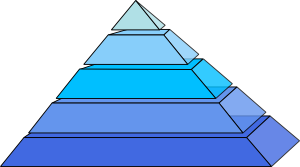
\includegraphics[width=1.1cm]{../Strukturfiler/FIGS/BluePyramid} & \begin{minipage}{\obsl}}{\end{minipage}\\ \end{tabular}\vspace{4mm}\newline}


% = Forudsætning = basis
\newenvironment{basis}{\begin{flushleft} \begin{itshape} }{\end{itshape} \end{flushleft}}


% = Opsummering =
\newenvironment{summary}{\clearpage\pagecolor{sumgul}\section{Opsummering}}{\newpage\pagecolor{white}}











% = Counter
\newcounter{opgavecount}[section]
\setcounter{opgavecount}{0}
\newcounter{spgcount}[opgavecount]
\setcounter{spgcount}{0}
\renewcommand{\thespgcount}{\alph{spgcount})}



% = EXERCISE = (DIVIDER)

\newcommand{\exercisebegin}[1][]{\bigskip\needspace{3\baselineskip}\refstepcounter{opgavecount}\titlegraphic{mingroen}\textcolor{mingroen}{\th{Opgave \theopgavecount \hspace*{1cm} #1}}\medskip\par}

% = QUIZEXERCISE = (DIVIDER)

\newcommand{\quizexercisebegin}[1][]{\bigskip\needspace{3\baselineskip}\refstepcounter{opgavecount}\titlegraphic{mingroen}\textcolor{mingroen}{\th{Quiz-Opgave \theopgavecount \hspace*{1cm} #1}}\medskip\par}

% = QUESTION =

\newenvironment{question}{\refstepcounter{spgcount}\begin{itemize}\item[\thespgcount]}{\end{itemize}\hspace*{\fill}}

% = VINK =

\newenvironment{vink}{\begin{tabular}{m{.9cm}<{\hspace*{2mm}}@{}|m{\obsl}@{}}\hspace*{-4pt}\raggedleft
\includegraphics[width=.9cm]{../Strukturfiler/FIGS/Think} & \begin{minipage}{\obsl}}{\end{minipage}\\ \end{tabular}\medskip\\}
	
% = FACIT =

\newenvironment{facit}{\begin{tabular}{m{.9cm}<{\hspace*{2mm}}@{}|m{\obsl}@{}}\hspace*{-4pt}\raggedleft
\includegraphics[width=.9cm]{../Strukturfiler/FIGS/Check} & \begin{minipage}{\obsl}}{\end{minipage}\\ \end{tabular}\medskip\\}








\newcommand{\afsnit}[1]{\bigskip\th{\titlegraphic{mingroen}\textcolor{mingroen}{#1}} \\ \rule[7pt]{.4\textwidth}{1pt} \vspace*{-2.5mm}\par}

% (DIVIDER):
\newcommand{\ugedagdatotitel}[4]{\pagebreak[4]\section{Semesteruge #1 -- #2 Dag \hspace*{1mm} (#3)} \vspace*{-4mm} \rule[5pt]{\textwidth}{1pt}\vspace*{-2.5mm} \begin{center}\large{\th{#4}}\end{center} \fancyhead[C]{\th{Semesteruge #1}}}

\newenvironment{skema}[1]{\definecolor{shadecolor}{rgb}{0.96,.98, 1.0} \setlength{\FrameSep}{6pt} \renewcommand{\FrameHeightAdjust}{10pt} \vspace*{-4pt}\begin{shaded} \begin{tabular}{#1}}{\end{tabular} \end{shaded} \vspace*{-7pt}}


% ========================

% MAKROER

%\newenvironment{matr}[1][]{\hspace*{-.8mm}\left[\hspace*{-1mm}\begin{array}{#1}}{\end{array}\hspace*{-1mm}\right]\hspace*{-.8mm}}
\newcommand{\bevisslut}{\begin{scriptsize} \begin{flushright} $ \blacksquare $ \end{flushright} \end{scriptsize}}

\newcommand{\tref}[2]{\hyperref[#1]{#2 \ref*{#1}}}
\newcommand{\thref}[2]{\hyperref[#1]{#2}}

\newcommand{\refA}[1]{\colorbox{yellow}{\ref{#1}}}
\newcommand{\hrefA}[2]{\colorbox{yellow}{\href{#1}{#2}}}
\newcommand{\trefA}[2]{\colorbox{yellow}{\hyperref[#1]{#2 \ref*{#1}}}}
\newcommand{\threfA}[2]{\colorbox{yellow}{\hyperref[#1]{#2}}}

\newenvironment{matr}[1]{\hspace*{-.8mm}\begin{bmatrix}\hspace*{-1mm}\begin{array}{#1}}{\end{array}\hspace*{-1mm}\end{bmatrix}\hspace*{-.8mm}}
\newcommand{\transp}{\hspace*{-.6mm}^{\top}}

\newcommand{\maengde}[2]{\left\lbrace \hspace*{-1mm} \begin{array}{c|c} #1 & #2 \end{array} \hspace*{-1mm} \right\rbrace}

\newenvironment{eqnalign}[1]{\setlength{\arraycolsep}{1.3pt}\begin{equation}\begin{array}{#1}}{\end{array}\end{equation}\par}
\newcommand{\eqnl}{\setlength{\arraycolsep}{1.3pt}}

\newcommand{\matind}[3]{{_\mathrm{#1}\mathbf{#2}_\mathrm{#3}}}
\newcommand{\vekind}[2]{{_\mathrm{#1}\mathbf{#2}}}
\newcommand{\jac}[2]{{\mathrm{Jacobi}_\mathbf{#1} (#2)}}
\newcommand{\diver}[2]{{\mathrm{div}\mathbf{#1} (#2)}}
\newcommand{\rot}[1]{{\mathbf{rot}\mathbf{(#1)}}}

\newcommand{\am}{\mathrm{am}}
\newcommand{\gm}{\mathrm{gm}}
\newcommand{\E}{\mathrm{E}}
\newcommand{\Span}{\mathrm{span}}
\newcommand{\mU}{\mathbf{U}}

\newcommand{\ms}{\medskip\\}
\newcommand{\bs}{\bigskip\\}

\newcommand{\mA}{\mathbf{A}}
\newcommand{\mB}{\mathbf{B}}
\newcommand{\mC}{\mathbf{C}}
\newcommand{\mD}{\mathbf{D}}
\newcommand{\mE}{\mathbf{E}}
\newcommand{\mF}{\mathbf{F}}
\newcommand{\mK}{\mathbf{K}}
\newcommand{\mI}{\mathbf{I}}
\newcommand{\mM}{\mathbf{M}}
\newcommand{\mN}{\mathbf{N}}
\newcommand{\mQ}{\mathbf{Q}}
\newcommand{\mT}{\mathbf{T}}
\newcommand{\mV}{\mathbf{V}}
\newcommand{\mW}{\mathbf{W}}
\newcommand{\mX}{\mathbf{X}}
\newcommand{\ma}{\mathbf{a}}
\newcommand{\mb}{\mathbf{b}}
\newcommand{\mc}{\mathbf{c}}
\newcommand{\md}{\mathbf{d}}
\newcommand{\me}{\mathbf{e}}
\newcommand{\mn}{\mathbf{n}}
\newcommand{\mr}{\mathbf{r}}
\newcommand{\mv}{\mathbf{v}}
\newcommand{\mw}{\mathbf{w}}
\newcommand{\mx}{\mathbf{x}}
\newcommand{\mxb}{\mathbf{x_{bet}}}
\newcommand{\my}{\mathbf{y}}
\newcommand{\mz}{\mathbf{z}}
\newcommand{\reel}{\mathbb{R}}
\newcommand{\mL}{\bm{\Lambda}} %Lambda-matrix
\newcommand{\mnul}{\bm{0}}
\newcommand{\trap}[1]{\mathrm{trap}(#1)}
\newcommand{\Det}{\operatorname{Det}}
\newcommand{\adj}{\operatorname{adj}}
\newcommand{\Ar}{\operatorname{Areal}}
\newcommand{\Vol}{\operatorname{Vol}}
\newcommand{\Rum}{\operatorname{Rum}}
\newcommand{\diag}{\operatorname{\bf{diag}}}
\newcommand{\bidiag}{\operatorname{\bf{bidiag}}}
\newcommand{\spanVec}[1]{\mathrm{span}\{#1\}}
\newcommand{\Div}{\operatorname{Div}}
\newcommand{\Rot}{\operatorname{\mathbf{Rot}}}

\newcommand{\Jac}{\operatorname{Jacobi}}
\newcommand{\Tan}{\operatorname{Tan}}
\newcommand{\Ort}{\operatorname{Ort}}
\newcommand{\Flux}{\operatorname{Flux}}
\newcommand{\Cmass}{\operatorname{Cm}}
\newcommand{\Imom}{\operatorname{Im}}
\newcommand{\Pmom}{\operatorname{Pm}}
\newcommand{\IS}{\operatorname{I}}
\newcommand{\IIS}{\operatorname{II}}
\newcommand{\IIIS}{\operatorname{III}}
\newcommand{\Le}{\operatorname{L}}
\newcommand{\app}{\operatorname{app}}
\newcommand{\M}{\operatorname{M}}
\newcommand{\re}{\mathrm{Re}}
\newcommand{\im}{\mathrm{Im}}

\newcommand{\compl}{\mathbb{C}} %de komplekse tal
\newcommand{\e}{\mathrm{e}} %eksponentialfunktionen. lodret 'e', og altså ikke kursiv ligesom andre bogstaver.





% Medialink: SCREEN: (QRcode) + thumbnail image + link på kodenummer (til qr.dtu.dk)
\newcommand{\onlinemedia}[3]{
	\begin{wrapfigure}{r}{3.2cm} 
		\vspace{-30pt} 
		\vspace{#1pt} 
		\begin{flushright} 
			\includegraphics[width=3cm]{qr/#2.png} 
			\tiny 
			\href{http://qr.dtu.dk/#2}{#2: #3}
			\normalsize  
		\end{flushright} 
		\vspace{-10pt} 
	\end{wrapfigure}
}
\newcommand{\onlinemediathumb}[3]{
	\begin{wrapfigure}{r}{3.2cm} 
		\vspace{-30pt} 
		\vspace{#1pt} 
		\begin{flushright} 
			\includegraphics[width=3cm]{qr/#2.png} 
			\includegraphics[width=3cm]{qr/#2_thumb.png} 
			\tiny 
			\href{http://qr.dtu.dk/#2}{#2: #3}
			\normalsize  
		\end{flushright} 
		\vspace{-10pt} 
	\end{wrapfigure}
}



% Index:
\usepackage{makeidx}
\makeindex
\newcommand\ind[2]{\index{#1}\textbf{\textit{\textcolor{black}{#2}}}}

% ###SERVER_EXCLUDE_BEGIN###
\externaldocument[NUID17-]{../../enoten/TN01-Talrum/Talrum}
\externaldocument[NUID1-]{../../enoten/TN02-Ligningssystemer/TNdriver}
\externaldocument[NUID2-]{../../enoten/TN03-Matricer_og_Matrixalgebra/Matricer_og_matrixalgebra}
\externaldocument[NUID3-]{../../enoten/TN04-Kvadratiske_matricer/TNdriver}
\externaldocument[NUID11-]{../../enoten/TN05-Determinanter/Determinanter}
\externaldocument[NUID12-]{../../enoten/TN06-GeometriskeVektorer/GeometriskeVektorer}
\externaldocument[NUID18-]{../../enoten/TN07-Vektorrum/VektorRum}
\externaldocument[NUID21-]{../../enoten/TN08-LinAfbildninger/LinAfbildninger}
\externaldocument[NUID23-]{../../enoten/TN09-Egenvaerdier_og_egenvektorer/TNdriver}
\externaldocument[NUID24-]{../../enoten/TN10-Diagonalisering_med_egenvektorer/TNdriver}
\externaldocument[NUID10-]{../../enoten/TN11-1.ordens_differentialligninger/TNdriver}
\externaldocument[NUID13-]{../../enoten/TN12-1.ordens_differentialligningssystemer/TNdriver}
\externaldocument[NUID14-]{../../enoten/TN13-2.ordens_differentialligninger/TNdriver}
\externaldocument[NUID27-]{../../enoten/TN14-Elemenataere_funktioner/Elementaere_Funktioner}
\externaldocument[NUID28-]{../../enoten/TN15-Funktioner2Variable/Funktioner_To_Variable}
\externaldocument[NUID29-]{../../enoten/TN16-Gradienter_og_Tangentplaner/Gradienter_og_Tangentplaner}
\externaldocument[NUID32-]{../../enoten/TN17-Taylor_formler/Taylor_Formler}
\externaldocument[NUID33-]{../../enoten/TN18-Taylor_2Var/Taylor_2Var}
\externaldocument[NUID34-]{../../enoten/TN19-SymMat/SymmetriskeMatricer}
\externaldocument[NUID35-]{../../enoten/TN20-KegleSnit/Keglesnit}
\externaldocument[NUID36-]{../../enoten/TN21-Riemann_Integral/Riemann_01}
\externaldocument[NUID37-]{../../enoten/TN22-Plan_Int/Plan_Int_01}
\externaldocument[NUID39-]{../../enoten/TN23-Flade_Int/Flade_Rum_Int_01}
\externaldocument[NUID40-]{../../enoten/TN24-Vektorfelter/Vektorfelter_01}
\externaldocument[NUID41-]{../../enoten/TN25-Flux/Flux_02}
\externaldocument[NUID42-]{../../enoten/TN26-Gauss/Gauss_01}
\externaldocument[NUID128-]{../../enoten/TN27-Stokes/Stokes_01}
\externaldocument[NUID43-]{../../enoten/TN29-KomplekseTal/KomplekseTal}

\externaldocument[NUID6-]{../../E-math-opgaver/Opgaver/opgU123}
\externaldocument[NUID19-]{../../E-math-opgaver/Opgaver/opgU45}
\externaldocument[NUID20-]{../../E-math-opgaver/Opgaver/opgU678}
\externaldocument[NUID25-]{../../E-math-opgaver/Opgaver/opgU910SD}
\externaldocument[NUID31-]{../../E-math-opgaver/OpgaverF11-U123/opgF123}
% \externaldocument[NUID9-]{../../E-math-opgaver/Opgaver/Dagsordner E10}
% ###SERVER_EXCLUDE_END###


% Begin document and set alternative chapter title:
\begin{document}
\renewcommand{\chaptername}{eNote}

\setcounter{chapter}{8} %SÆT DETTE TAL TIL 1 MINDRE END DET AKTUELLE TRANSFERNOTE-NUMMER!!

%%%%%%%%%%%%%%%%%%%%%%%%%%%%%%%%%%%%%%%%%%%%%
%%%%%%%%%%%%%%%%%%%%%%%%%%%%%%%%%%%%%%%%%%%%%
%%% HERFRA SKAL DU SKRIVE ELLER INDSÆTTE %%%%
%%% DEN FIL DU ØNSKER %%%%%%%%%%%%%%%%%%%%%%%
%%%%%%%%%%%%%%%%%%%%%%%%%%%%%%%%%%%%%%%%%%%%%
%%%%%%%%%%%%%%%%%%%%%%%%%%%%%%%%%%%%%%%%%%%%%

\chapter{Egenværdier og egenvektorer} \label{tn9}

\begin{basis}
Denne note indfører begreberne egenværdier og egenvektorer for lineære afbildninger i vilkårlige generelle vektorrum og går derefter i dybden med egenværdier og egenvektorer til kvadratiske matricer. Noten bygger derfor på viden omkring generelle vektorrum, se \tref{NUID18-tn7}{eNote}, på viden om algebra med matricer, se \tref{NUID2-tn3}{eNote} og \tref{NUID3-tn4}{eNote}, og på viden om lineære afbildninger se \tref{NUID21-tn8}{eNote}.
\end{basis}

\section{Egenværdiproblemet for lineære afbildninger}

\subsection{Indledning}

I denne eNote betragter vi lineære afbildninger af typen 
\begin{equation}\label{fiksektor}
f:V\rightarrow V
\end{equation}
 det vil sige lineære afbildninger hvor \textit{definitionsrummet} og \textit{dispositionsrummet} er det samme vektorrum. Dette åbner op for et særligt fænomen, at en vektor kan være identisk med sin billedvektor:
\begin{equation}\label{fiksektor}
f(\mv)=\mv\,.
\end{equation}
Vektorer af denne type kaldes \textit{fiksvektorer} for $f\,$. Mere generelt er vi på jagt efter \textit{egenvektorer}, det vil sige vektorer som er proportionale med deres billedvektorer. Man taler i denne forbindelse om \textit{egenværdiproblemet}: at finde en skalar $\lambda\,$ og en egentlig vektor $\mv$ som opfylder vektorligningen: 
\begin{equation}\label{egenvektor}
f(\mv)=\lambda\mv\,.
\end{equation}
Hvis $\lambda\,$ er en skalar og $\mv$ en egentlig vektor som opfylder \ref{egenvektor} kaldes proportionalitetfaktoren $\lambda$ en \textit{egenværdi} for $f$ og $\mv$ en til $\lambda$ hørende \textit{egenvektor}. Lad os som eksempel tage en lineær afbildning 
$ f:G_3 \rightarrow G_3 $, det vil sige en lineær afbildning af mængden af rumvektorer ind sig selv, som afbilder tre givne vektorer som vist på figur 9.1.
\begin{center}
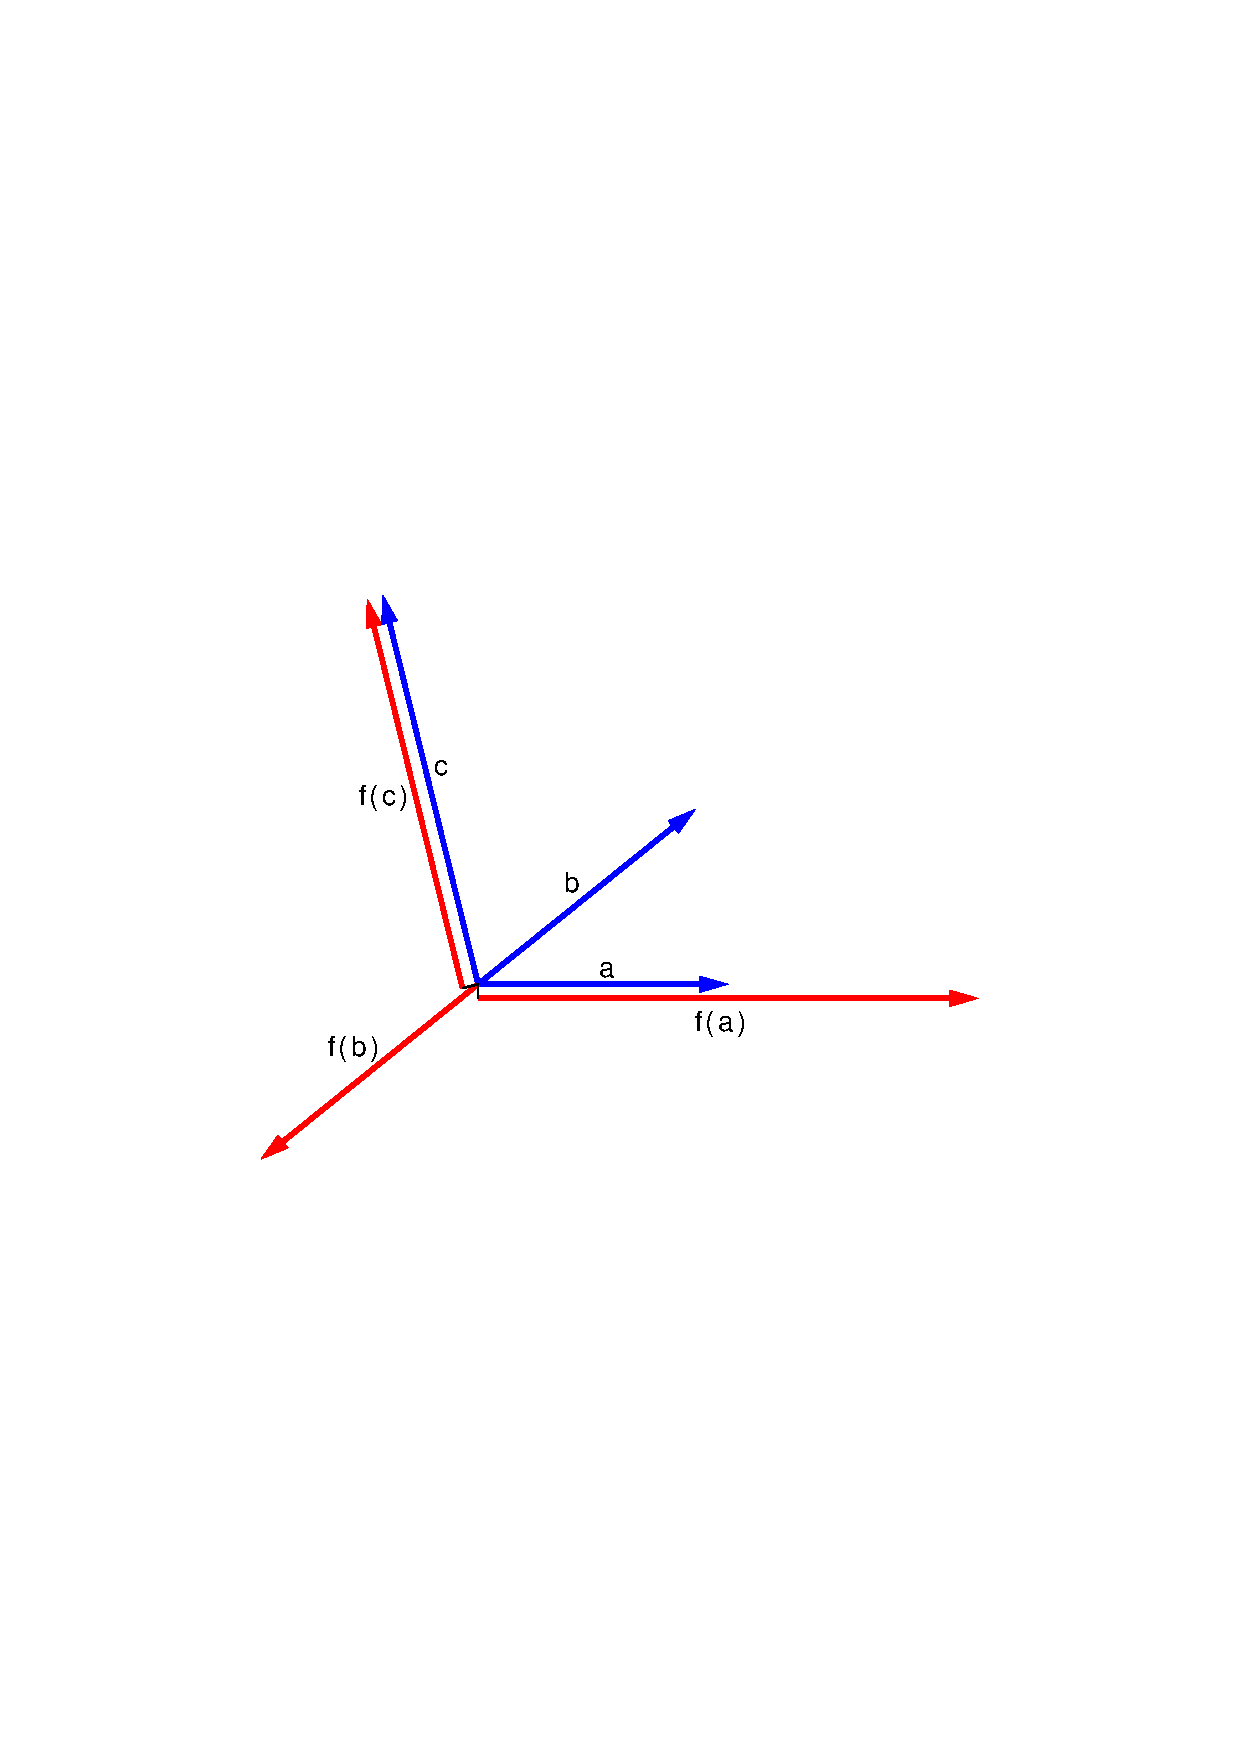
\includegraphics[trim=4.5cm 9.5cm 4.5cm 10cm,width=0.40\textwidth,clip]{evektorRummet.pdf} \\
Figur 9.1: Tre egenvektorer i rummet og deres billedvektorer. 	
\end{center}

Som antydet på figuren 9.1 er $\,f(\ma)=2\ma\,$. Derfor er $\,2\,$ en egenværdi for $f$ med tilhørende egenvektor $\,\ma\,$. Da endvidere $\,f(\mb)=-\mb\,$, er også $\,-1\,$ en egenværdi for $f$ med tilhørende egenvektor $\,\mb\,$. Og da endelig $\,f(\mc)=\mc\,$, er 1 en egenværdi for $f$ med tilhørende egenvektor $\,\mc\,$. Specielt er $\,\mc\,$ en fiksvektor for $f$.\bs
At løse egenværdiproblemer for lineære afbildninger er en af de mest afgørende problemstillinger i ingeniørmæssige anvendelser af lineær algebra. Dette hænger snævert sammen med at en lineær afbildning, hvis afbildningsmatrix med hensyn til en given basis er en \textit{diagonalmatrix}, er særlig enkel at overskue og arbejde med. Og her gælder der den komfortable regel, at hvis man vælger en basis bestående af egenvektorer for afbildningen, så bliver afbildningsmatricen automatisk en diagonalmatrix.\bs

I det følgende eksempel illustrerer vi disse pointer ved hjælp af lineære afbildninger i planen.

\begin{example}[Egenværdier og egenvektorer i planen]\label{drejningAfHuse}
Vektorrummet af vektorer i planen har symbolet $G_2(\reel)\,.$ Vi betragter en lineær afbildning
\begin{equation}\label{G3_egenvektorEks}
f:G_2(\reel)\rightarrow G_2(\reel)
\end{equation}
af mængden af plane vektorer ind i sig selv, som med hensyn til en given basis $(\ma_1,\ma_2)$ har følgende diagonalmatrix som afbildningsmatrix:
\begin{equation}\label{2x2diagM}
\matind aFa=\begin{matr}{rr}2&0\\0&3\end{matr}\,.
\end{equation}
Da der gælder at 
\begin{equation*}
_\mathrm{a}f(\ma_1)=\begin{matr}{rr}2&0\\0&3\end{matr}\,\begin{matr}{r}1\\0\end{matr}=\begin{matr}{r}2\\0\end{matr}=
2\cdot\begin{matr}{r}1\\0\end{matr}\end{equation*}
og
\begin{equation*}
_\mathrm{a}f(\ma_2)=\begin{matr}{rr}2&0\\0&3\end{matr}\,\begin{matr}{r}0\\1\end{matr}=
\begin{matr}{r}0\\3\end{matr}=
3\cdot\begin{matr}{r}0\\1\end{matr}\,
\end{equation*}
har vi at $\,f(\ma_1)=2\ma_1\,$ og $\,f(\ma_2)=3\ma_2\,$. Begge basisvektorer er altså egenvektorer for $f\,$, idet $\,\ma_1\,$ tilhører egenværdien $\,2\,$, og $\,\ma_2\,$ tilhører egenværdien $\,3\,$. Egenværdierne er diagonalelementerne i $\,\matind aFa\,$.\\

Vi betragter nu en vilkårlig vektor $\,\mathbf x=x_1\ma_1+x_2\ma_2\,$ og finder dens billedvektor: 
\begin{equation*}
_\mathrm{a}f(\mathbf x)=\begin{matr}{rr}2&0\\0&3\end{matr}\,\begin{matr}{r}x_1\\x_2\end{matr}=\begin{matr}{r}2x_1\\3x_2\end{matr}\,.
\end{equation*}
Ved afbildningen bliver $x_1$-koordinaten ganget med egenværdien 2, mens $x_2$-koordinaten bliver ganget med egenværdien 3. Geo\-metrisk betyder dette at hele planen ved afbildningen ``strækkes'' først med faktoren 2 i retningen $\,\ma_1\,$ og dernæst faktoren 3 i retningen $\,\ma_2\,$, se virkningen på en vilkårligt valgt vektor $\,\mathbf x \,$ på figur 9.2.

\begin{center}
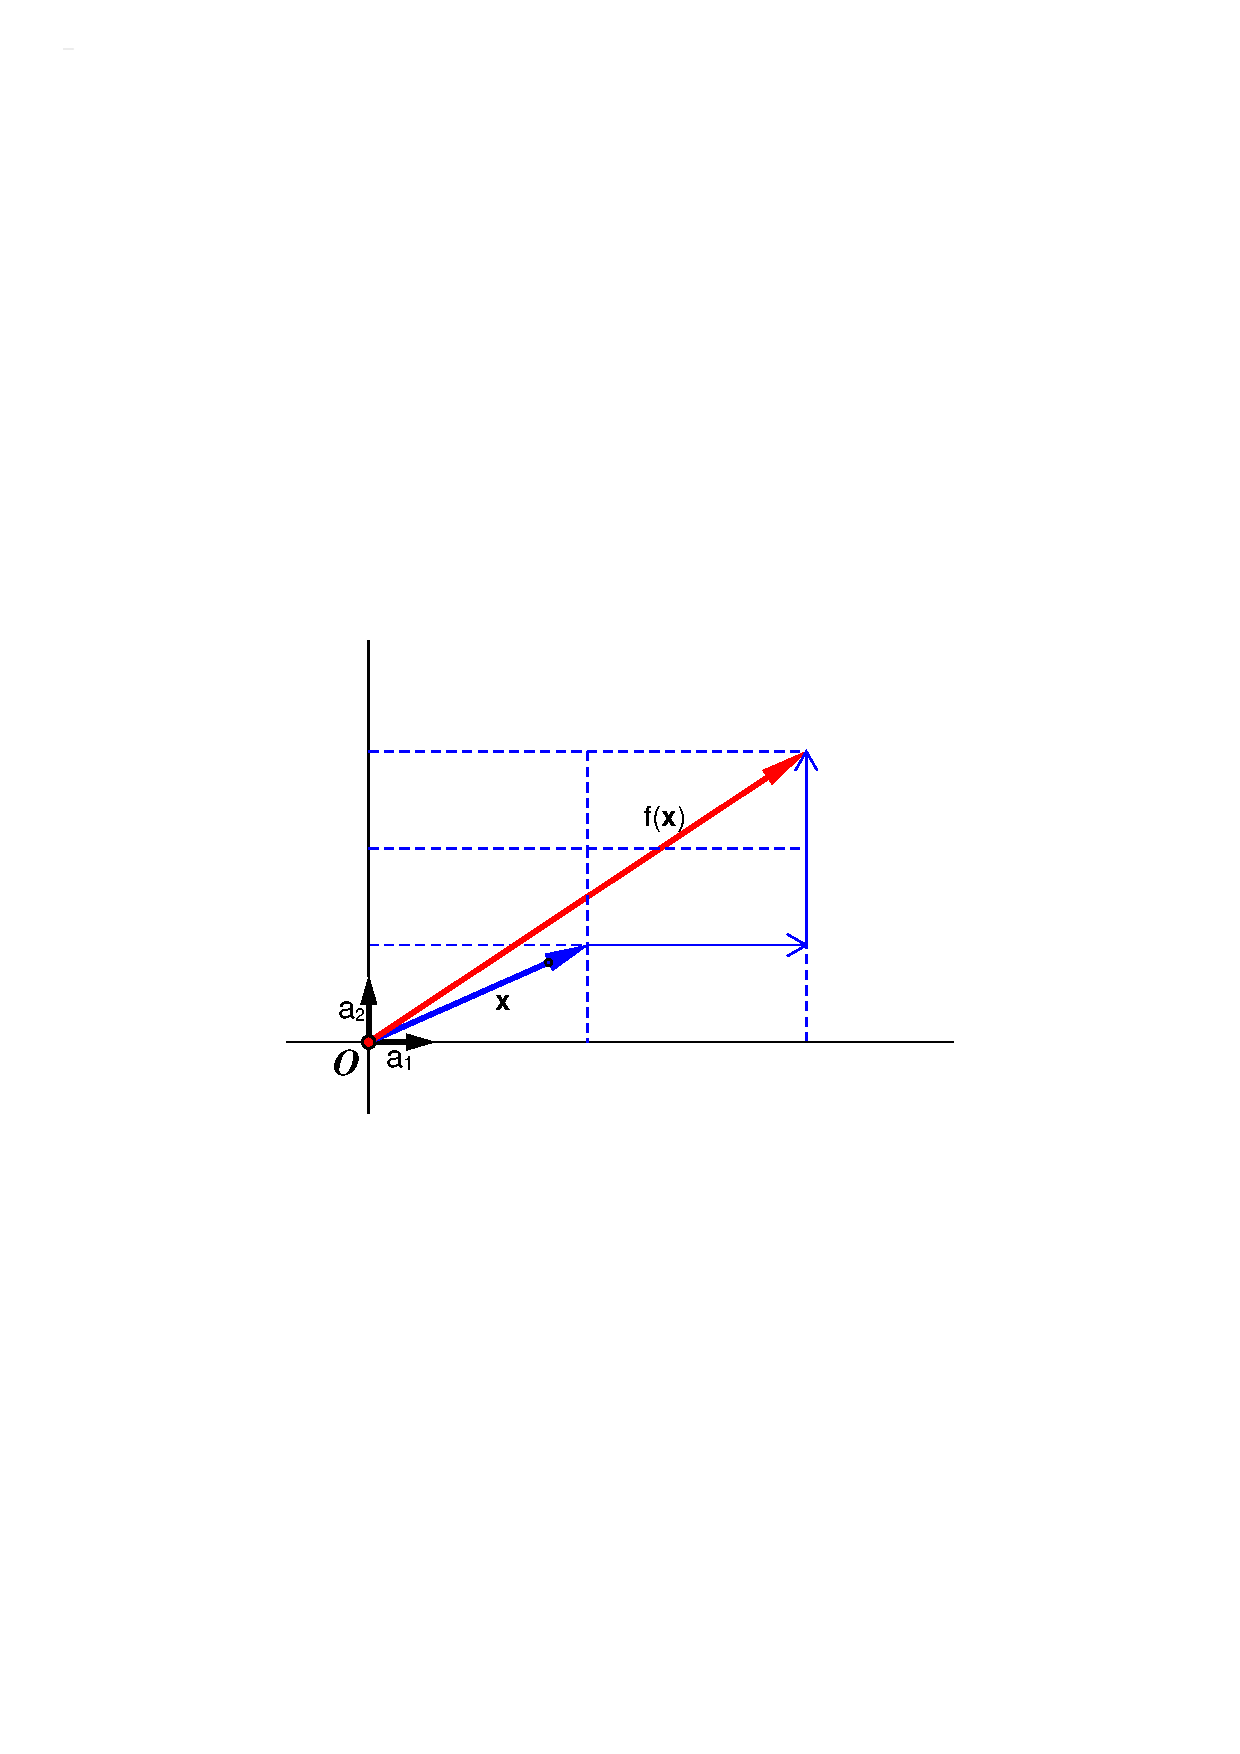
\includegraphics[trim=4.5cm 10.5cm 4.5cm 10.5cm,width=0.40\textwidth,clip]{diagMatrix.pdf} \\
Figur 9.2: Vektoren $\,\mathbf x\,$ strækkes vandret med faktor 2 og lodret med faktor 3.
\end{center}

På figur 9.3 har vi valgt standardbasen $\,(\mathbf i,\mathbf j)\,$ og illustrerer hvordan den lineære afbildning $g$ som har afbildningsmatricen 
\begin{equation*}
\matind eGe=\begin{matr}{rr}2&0\\0&3\end{matr}\,,
\end{equation*}
afbilder det ``blå hus'' over i det ``røde hus'' ved at alle stedvektorer til punkter i ``blå hus'' strækkes med faktoren 2 i vandret retning og med faktoren 3 i lodret retning.
\begin{center}
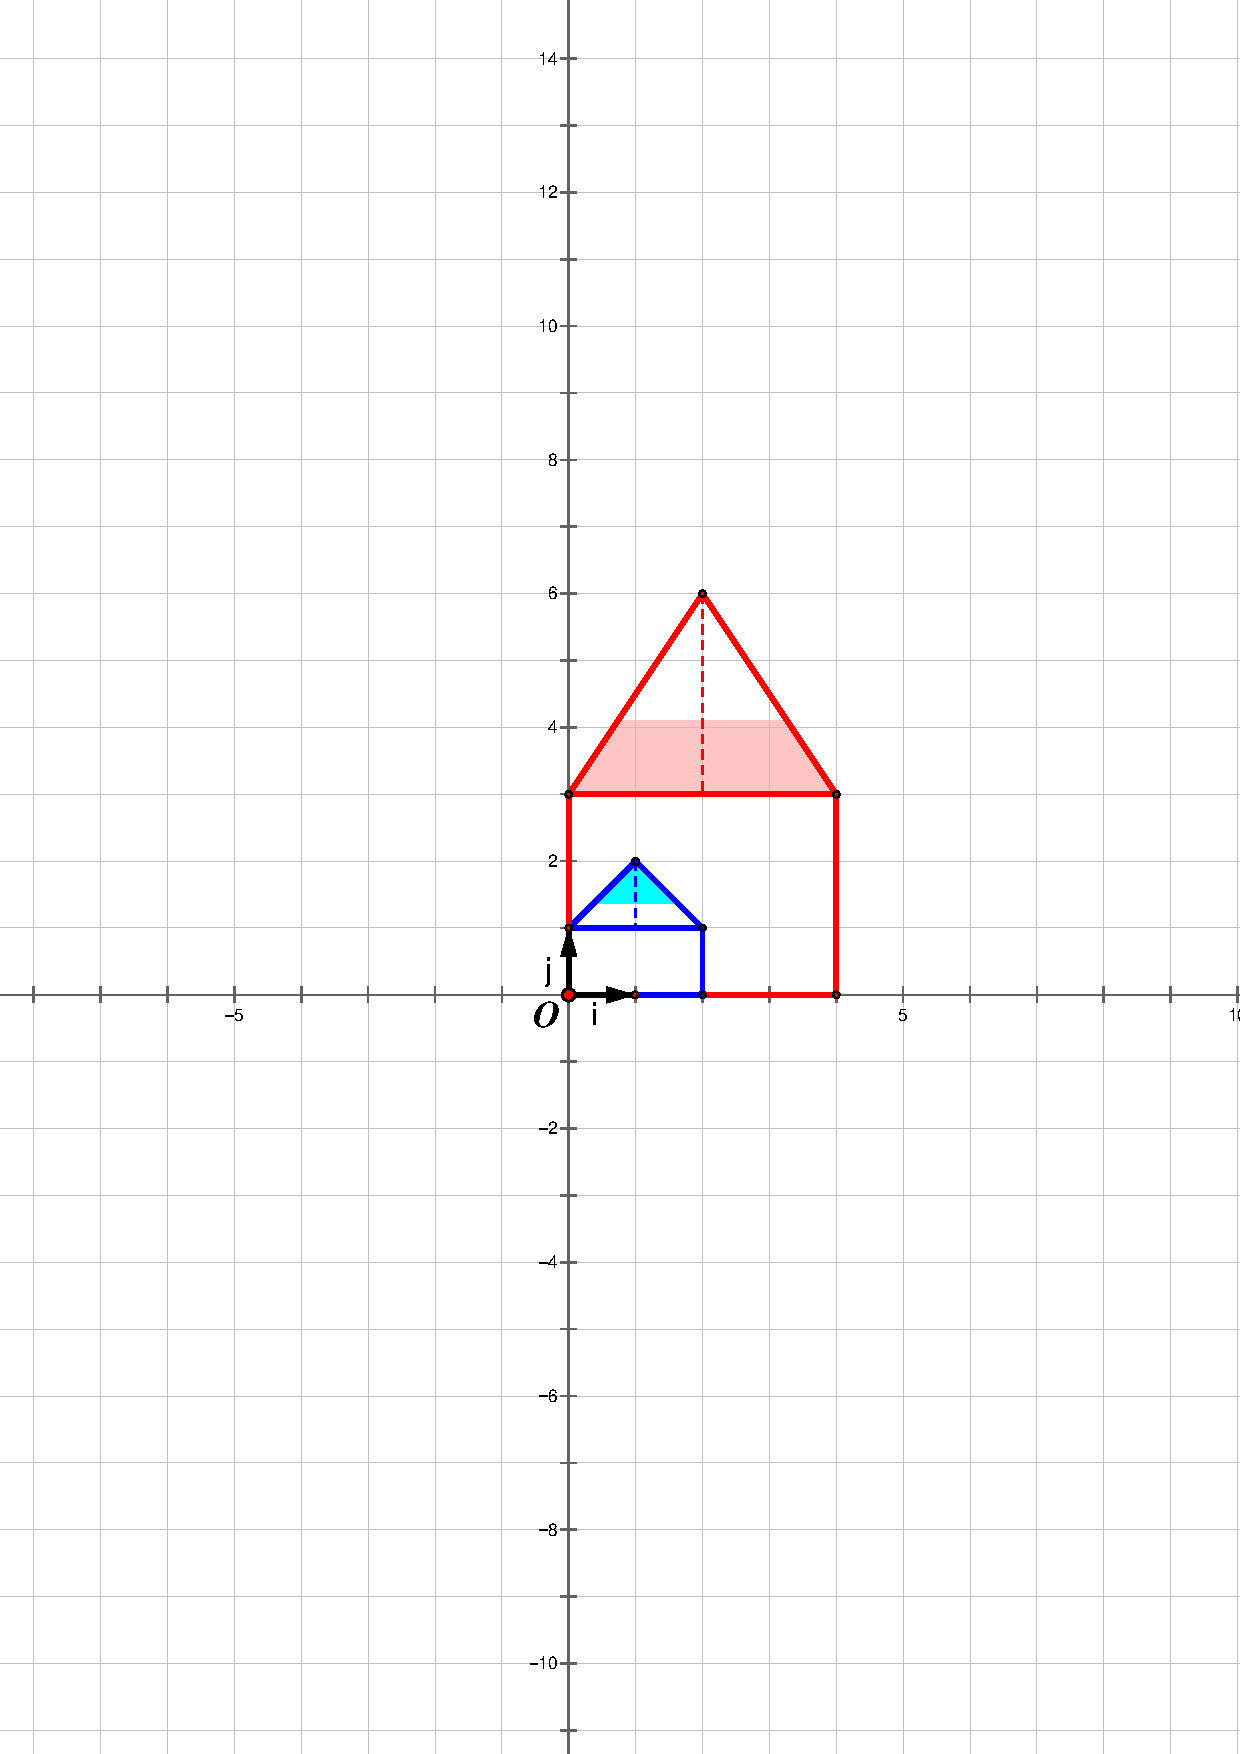
\includegraphics[trim=8cm 11.4cm 5.3cm 9.4cm,width=0.30\textwidth,clip]{Hus2.pdf} \\
Figur 9.3: Det blå hus strækkes vandret med faktor 2 og lodret med faktor 3.	
\end{center}

Vi undersøger nu en anden lineær afbildning $\,h\,$ hvis afbildningsmatrix med hensyn til standardbasen ikke er en diagonalmatrix:
\begin{equation*}
\matind eHe=\begin{matr}{rr}7/3&2/3\\1/3&8/3\end{matr}\,.
\end{equation*}
Her kan man ikke straks afgøre om afbildningen er sammensat af to strækninger i to givne retninger. Og man får ikke umiddelbart hints ved at afbilde
det blå hus fra figur 9.4 ved hjælp af $\,h\,$:
\begin{center}
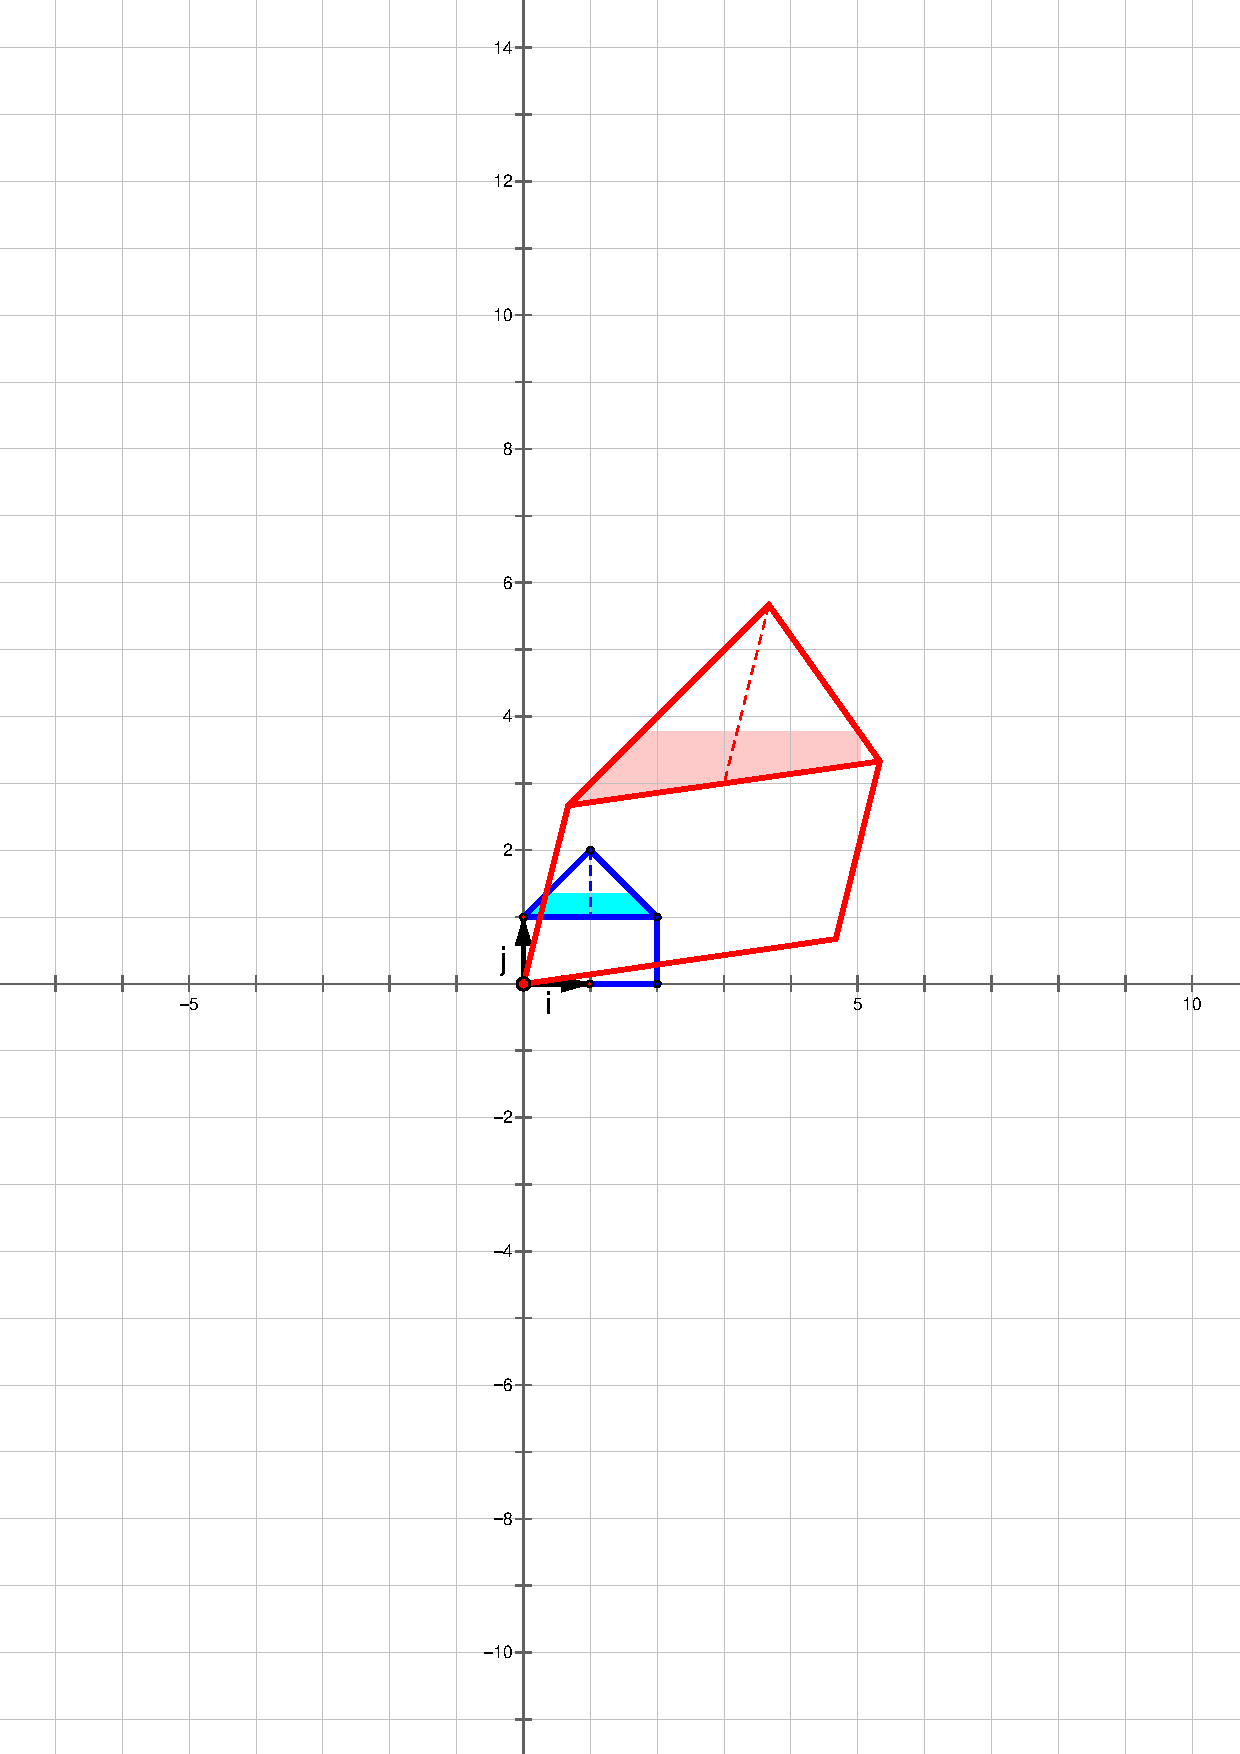
\includegraphics[trim=8cm 11.6cm 5.3cm 9.4cm,width=0.30\textwidth,clip]{Hus3.pdf} \\
Figur 9.4: Hus	
\end{center}
Men faktisk er det også i tilfældet $\,h\,$ muligt at vælge en basis som består af to lineært uafhængige egenvektorer for $\,h\,$. Lad nemlig $\,\mb_1\,$ være givet ved $e$-koordinaterne $(2,-1)$ og $\,\mb_2\,$ ved $e$-koordinaterne $(1,1)\,$. Så gælder der
\begin{equation*}
_\mathrm{e}h(\mb_1)=\begin{matr}{rr}7/3&2/3\\1/3&8/3\end{matr}\,\begin{matr}{r}2\\-1\end{matr}=\begin{matr}{r}4\\-2\end{matr}
=2\cdot\begin{matr}{r}2\\-1\end{matr}
\end{equation*}
og
\begin{equation*}
_\mathrm{e}h(\mb_2)=\begin{matr}{rr}7/3&2/3\\1/3&8/3\end{matr}\,\begin{matr}{r}1\\1\end{matr}=\begin{matr}{r}3\\3\end{matr}
=3\cdot\begin{matr}{r}1\\1\end{matr}\,.
\end{equation*}
Der gælder med andre ord
at $\,h(\mb_1)=2\mb_1\,$ og $\,h(\mb_2)=3\mb_2\,$. 
Vi ser at $\,\mb_1\,$ og $\,\mb_2\,$ er egenvektorer for $\,h\,$, og når vi vælger $(\mb_1,\mb_2)$ som basis, får afbildningsmatricen for $\,h\,$ med hensyn til denne basis formen: 
\begin{equation*}
\matind bGb=\begin{matr}{rr}2&0\\0&3\end{matr}\,.
\end{equation*}
Det viser sig dermed overraskende at afbildningsmatricen for $\,h\,$ også kan skrives på formen (\ref{2x2diagM}). Afbildningen $\,h\,$ er også sammensat af to strækninger med faktorerne 2 og 3. Blot er de to stræknings\textit{retninger} nu bestemt ved egenvektorerne $\,\mb_1\,$ og $\,\mb_2\,$. Dette ses tydeligere hvis vi afbilder et nyt blåt hus hvis hovedlinjer er parallelle med $b$-basisvektorerne:
\begin{center}
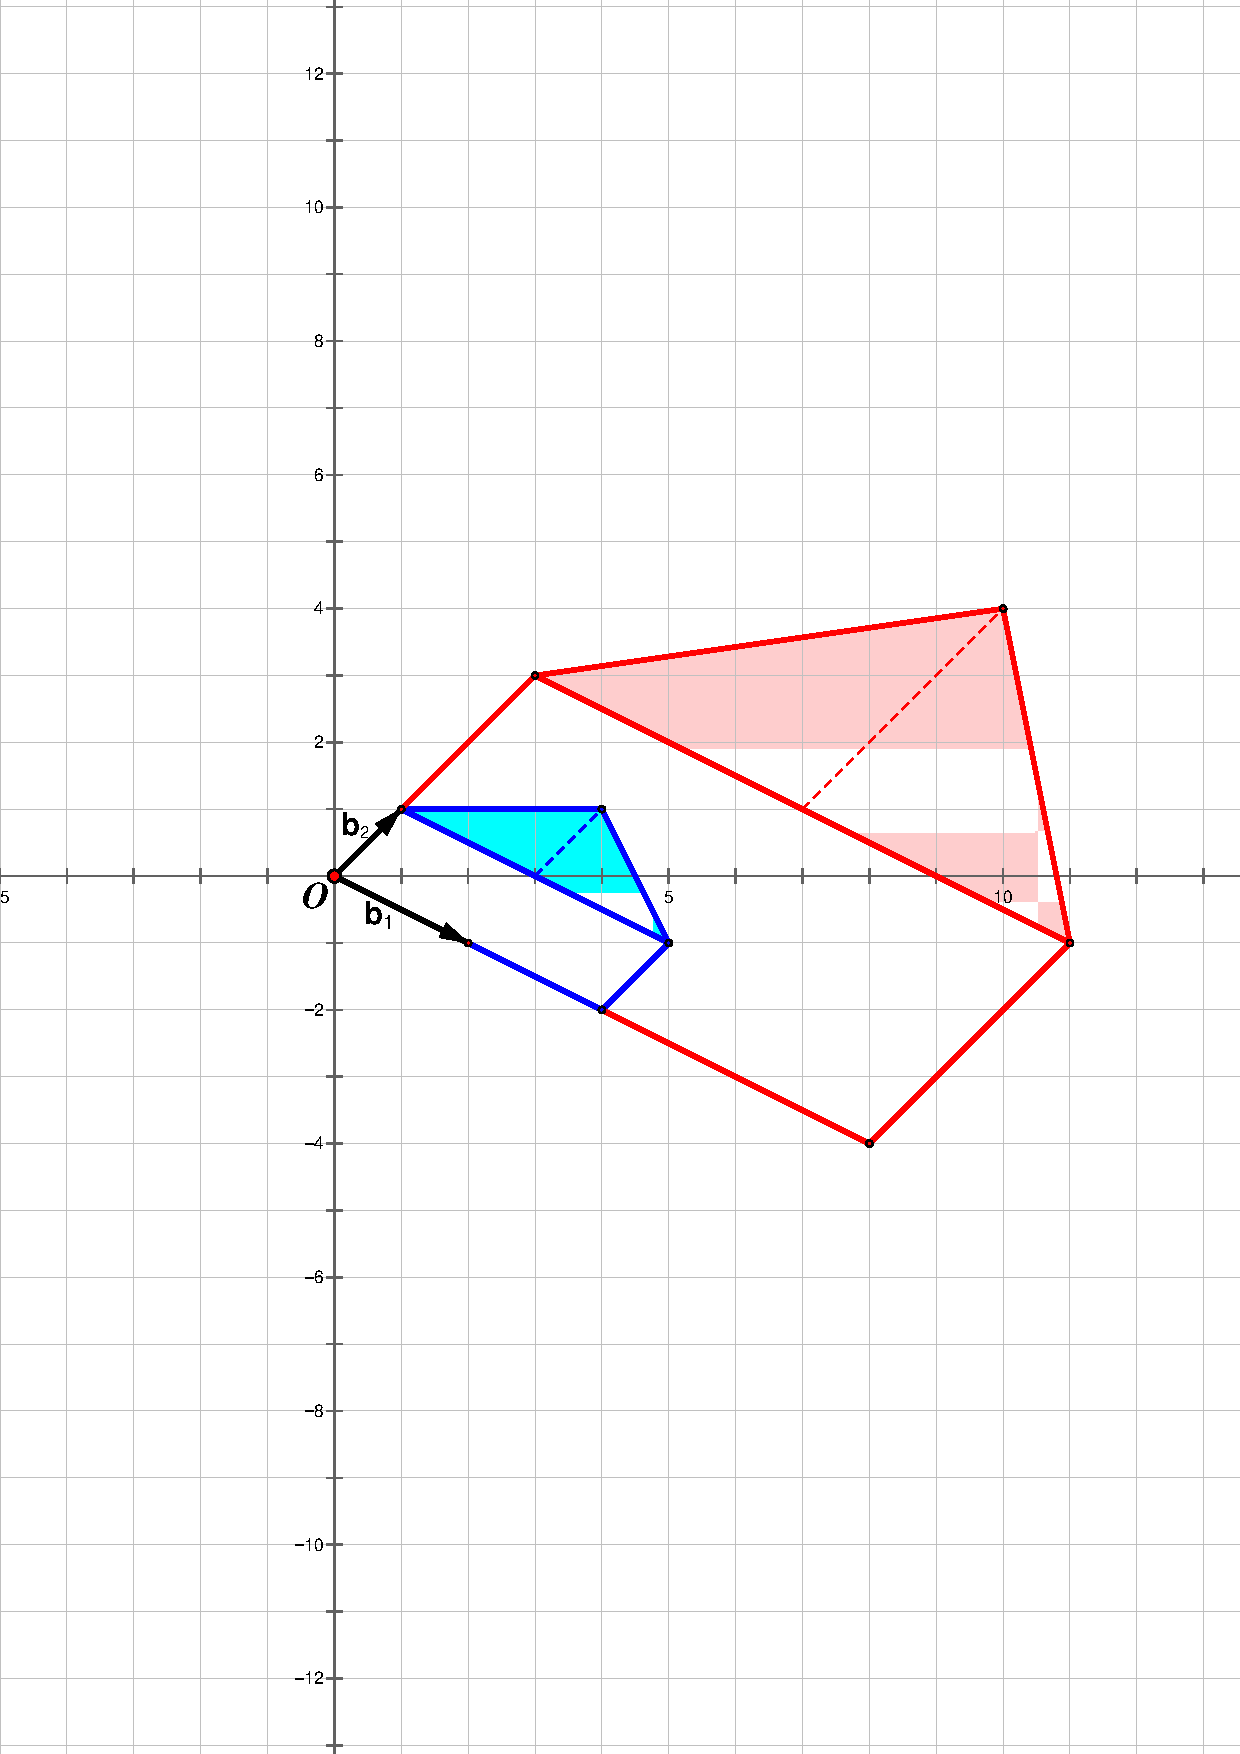
\includegraphics[trim=4.5cm 9.5cm 2cm 9cm,width=0.50\textwidth,clip]{Husdrejet2.pdf} \\
Figur 9.5: Det blå hus strækkes med faktor 2 hhv. faktor 3 i egenvektorernes retning	
\end{center}

Vi har hermed eksemplificeret: Hvis man kan finde to lineært uafhængige egenvektorer for en lineær afbildning i planen er det muligt
\begin{enumerate}
\item
at skrive dens afbildningsmatrix på diagonalform ved at vælge egenvektorerne som basis
\item 
at beskrive afbildningen som strækninger i egenvektorernes retninger med deres tilhørende egenværdier som strækningsfaktorer.
\end{enumerate}
\end{example}

\subsection{Egenværdier og deres tilhørende egenvektorer}

\textit{Egenværdiproblemet} for en lineær afbildning går i korthed ud på at besvare spørgsmålet: findes der egentlige vektorer hvis billedvektor er proportionale med vektoren selv. Det korte svar er at det kan man ikke svare generelt på, det afhænger af den enkelte afbildning. I det følgende forsøger vi at indkredse hvad vi faktisk kan sige generelt om egenværdiproblemet .

\begin{definition}[Egenværdi og egenvektor]\label{defE_values}
Lad $\,f:V\rightarrow V\,$ være en lineær afbildning af vektorrummet $\,V\,$ ind i sig selv. Hvis der findes en egentlig vektor $\mv\in V$ og en skalar $\lambda$, således at
\begin{equation}\label{egenvektor2}
f(\mv)=\lambda\mv\,,
\end{equation}
så kaldes proportionalitetsfaktoren $\lambda$ for en \textit{egenværdi} for $f$, mens $\mv$ kaldes for en \textit{egenvektor} som hører til $\lambda$.
\end{definition}

\begin{aha}
Hvis det ikke i definition \ref{defE_values} var krævet at der skulle findes en \textit{egentlig} vektor som opfylder $f(\mv)=\lambda\mv\,,$ ville enhver skalar $\lambda$ være en egenværdi, idet der jo for enhver skalar $\lambda$ gælder $\,f(\mnul)=\lambda\,\mnul\,.$  Men bemærk at \textit{hvis} $\lambda$ er en egenværdi, så \textit{er} nul-vektoren en egenvektor hørende til $\lambda\,$.
\end{aha}

\begin{aha}
Tallet $0$ kan godt være en egenværdi. Det kræver blot at der findes en egentligt vektor $\mv$ som opfylder $f(\mv)=\mnul\,$, da vi så har $f(\mv)=0\mv\,$.
\end{aha}

Hvis en lineær afbildning $f$ har blot én egenvektor $\,\mv\,$, så har den uendeligt mange egenvektorer. Dette er en simpel konsekvens af den følgende sætning. 

\begin{theorem}[Underrum af egenvektorer]\label{thLambdaUrum}
Hvis $\lambda$ er en egenværdi for en lineær afbildning $\,f:V\rightarrow V\,$, så er mængden af egenvektorer som hører til $\lambda\,$, et underrum i $V$.
\end{theorem}
\begin{bevis}
Lad $\,f:V\rightarrow V\,$ være en lineær afbildning af vektorrummet $V$ ind i sig selv, og antag at $\lambda$ er en egenværdi for $f\,.$ Vi skal vise at mængden af egenvektorer som hører til $\lambda$, opfylder de to stabilitetskrav for underrum, se \tref{NUID18-tn7.stabilNok}{sætning}. Lad $k$ være en vilkårlig skalar, og lad $\mathbf u$ og $\mv$ være to vilkårlige egenvektorer som hører til $\lambda$. Så gælder der under anvendelse af $L_1$:
$$
f(\mathbf u+\mv)=f(\mathbf u)+f(\mv)=\lambda\mathbf u+    \lambda \mv=\lambda(\mathbf u+\mv)\,.
$$
Sumvektoreren $\mathbf u+\mv$ er dermed en egenvektor hørende til $\lambda\,,$ og vi har hermed vist at egenvektorerne hørende til $\lambda$ opfylder stabilitetskravet vedrørende addition. Endvidere gælder der under anvendelse af $L_2$:
$$
f(k\mathbf u) = k f(\mathbf u)= k( \lambda \mathbf u)=\lambda(k\mathbf u)\,.
$$
Hermed vist at egenvektorerne hørende til $\lambda$ også opfylder stabilitetskravet vedrørende multiplikation med skalar. Samlet er det vist at mængden af egenvektorer som hører til en given egenværdi $\lambda$, er et underrum i definitionsrummet.
\end{bevis}

Sætning \ref{thLambdaUrum} giver anledning til den følgende definition:

\begin{definition}[Egenvektorrum]\label{defErum}
Lad $\,f:V \rightarrow V\,$ være en lineær afbildning af vektorrummet $V$ ind i sig selv, og lad $\lambda$ være en egenværdi for $f\,.$ \\

Ved \textit{egenvektorrummet} (eller kort \textit{egenrummet})  $\,E_{\lambda}\,$ hørende til $\lambda$ forstås underrummet af egenvektorer som hører til hører til $\lambda\,$:
$$
E_{\lambda}=\left\{\mv\in V\,|\,\,f(\mv)=\lambda \mv\,\right\}\,.$$
Hvis $\,E_{\lambda}\,$ er endeligt-dimensionalt, kaldes dim$(E_{\lambda})$ for den \textit{geometriske multiplicitet} af $\,\lambda\,$, betegnet $ \gm(\lambda) $.
\end{definition}

I det følgende eksempel betragtes en lineær afbildning som har to egenværdier, begge med geometrisk multiplicitet $\,1\,$. 
\begin{example}[Egenrum for spejling]\label{spejling}
I planen er der tegnet en ret linje $m$ gennem Origo. Med $s$ betegnes den lineære afbildning der afbilder en vektor $\mv$, afsat ud fra Origo, i dens spejling $s(\mv)$ i $\,m\,$, se figur 9.5:
\begin{center}
		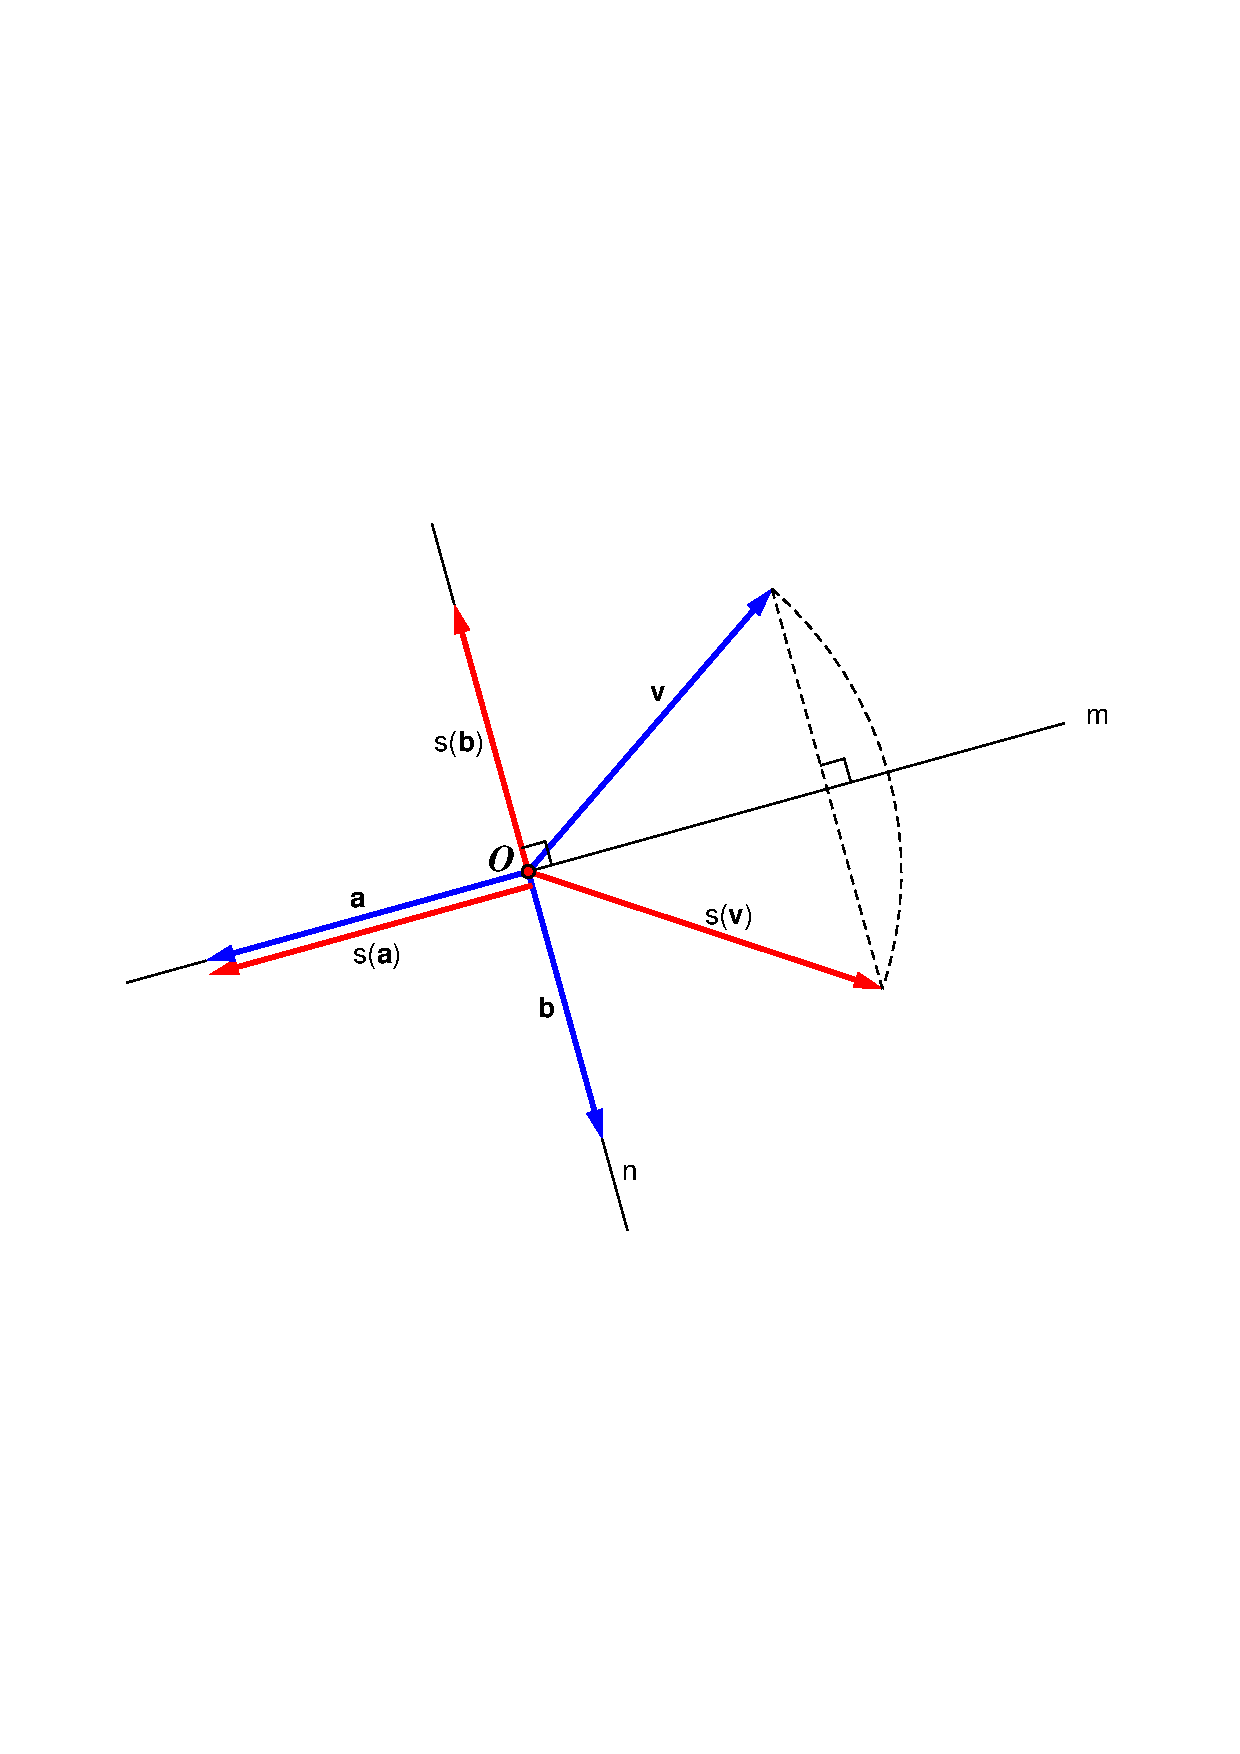
\includegraphics[trim=2cm 9.2cm 2cm
 9cm,width=0.6\textwidth,clip]{evSpejling.pdf}
  \\Figur 9.5: Egenværdiproblemet for spejling i $m\,$. 
\end{center}
Lad $\ma$ være en vilkårlig egentlig vektor som ligger på $m$. Da der gælder $$s(\ma)=\ma=1\cdot \ma\,$$ er $\,1\,$ en egenværdi for $\,s\,$. Egenrummet $\,E_1\,$ er mængden af vektorer som ligger på $\,m\,$.\\

Vi tegner nu en ret linje $\,n\,$ gennem Origo, vinkelret på $\,m\,$. Lad $\mb$ være en vilkårlig egentlig vektor som ligger på $n$. Da der gælder $$s(\mb)=-\mb=(-1)\cdot \mb\,,$$ er $\,-1\,$ en egenværdi for $s\,$. Egenrummet $\,E_{-1}\,$ er mængden af vektorer som ligger på $\,n\,$.
\end{example}

At ikke alle lineære afbildninger har egenværdier og dermed egenvektorer, fremgår af det følgende eksempel.

\begin{example}\label{hatvektor}
Lad os undersøge egenværdiproblemet for den lineære afbildning $f:G_2\rightarrow G_2$ som til en egentlig vektor $\mv$ i planen knytter dens tværvektor:
$$f(\mv)=\widehat{\mv}\,.$$
Da en egentlig vektor $\mv$ aldrig kan være proportional (parallel) med sin tværvektor, må der for ethvert valg af en skalar $\lambda$ nødvendigvis gælde at
$$\widehat{\mv}\neq \lambda \mv\,.$$
Derfor findes der ikke egenværdier og dermed heller ikke egenvektorer for $f\,$.
\end{example}


Af den følgende opgave fremgår blandt andet at dimensionen af et egenvektorrum meget vel kan være større end 1. 

\begin{exercise}\label{evProjektion}
I rummet er der givet et standard $\,(O,\mathbf i,\mathbf j,\mathbf k)$-koordinatsystem. Alle vektorer tænkes afsat ud fra Origo. Afbildningen $\,p\,$ projicerer vektorer ned i $(X,Y)$-planen i rummet, se figur 9.6.

\begin{center}
		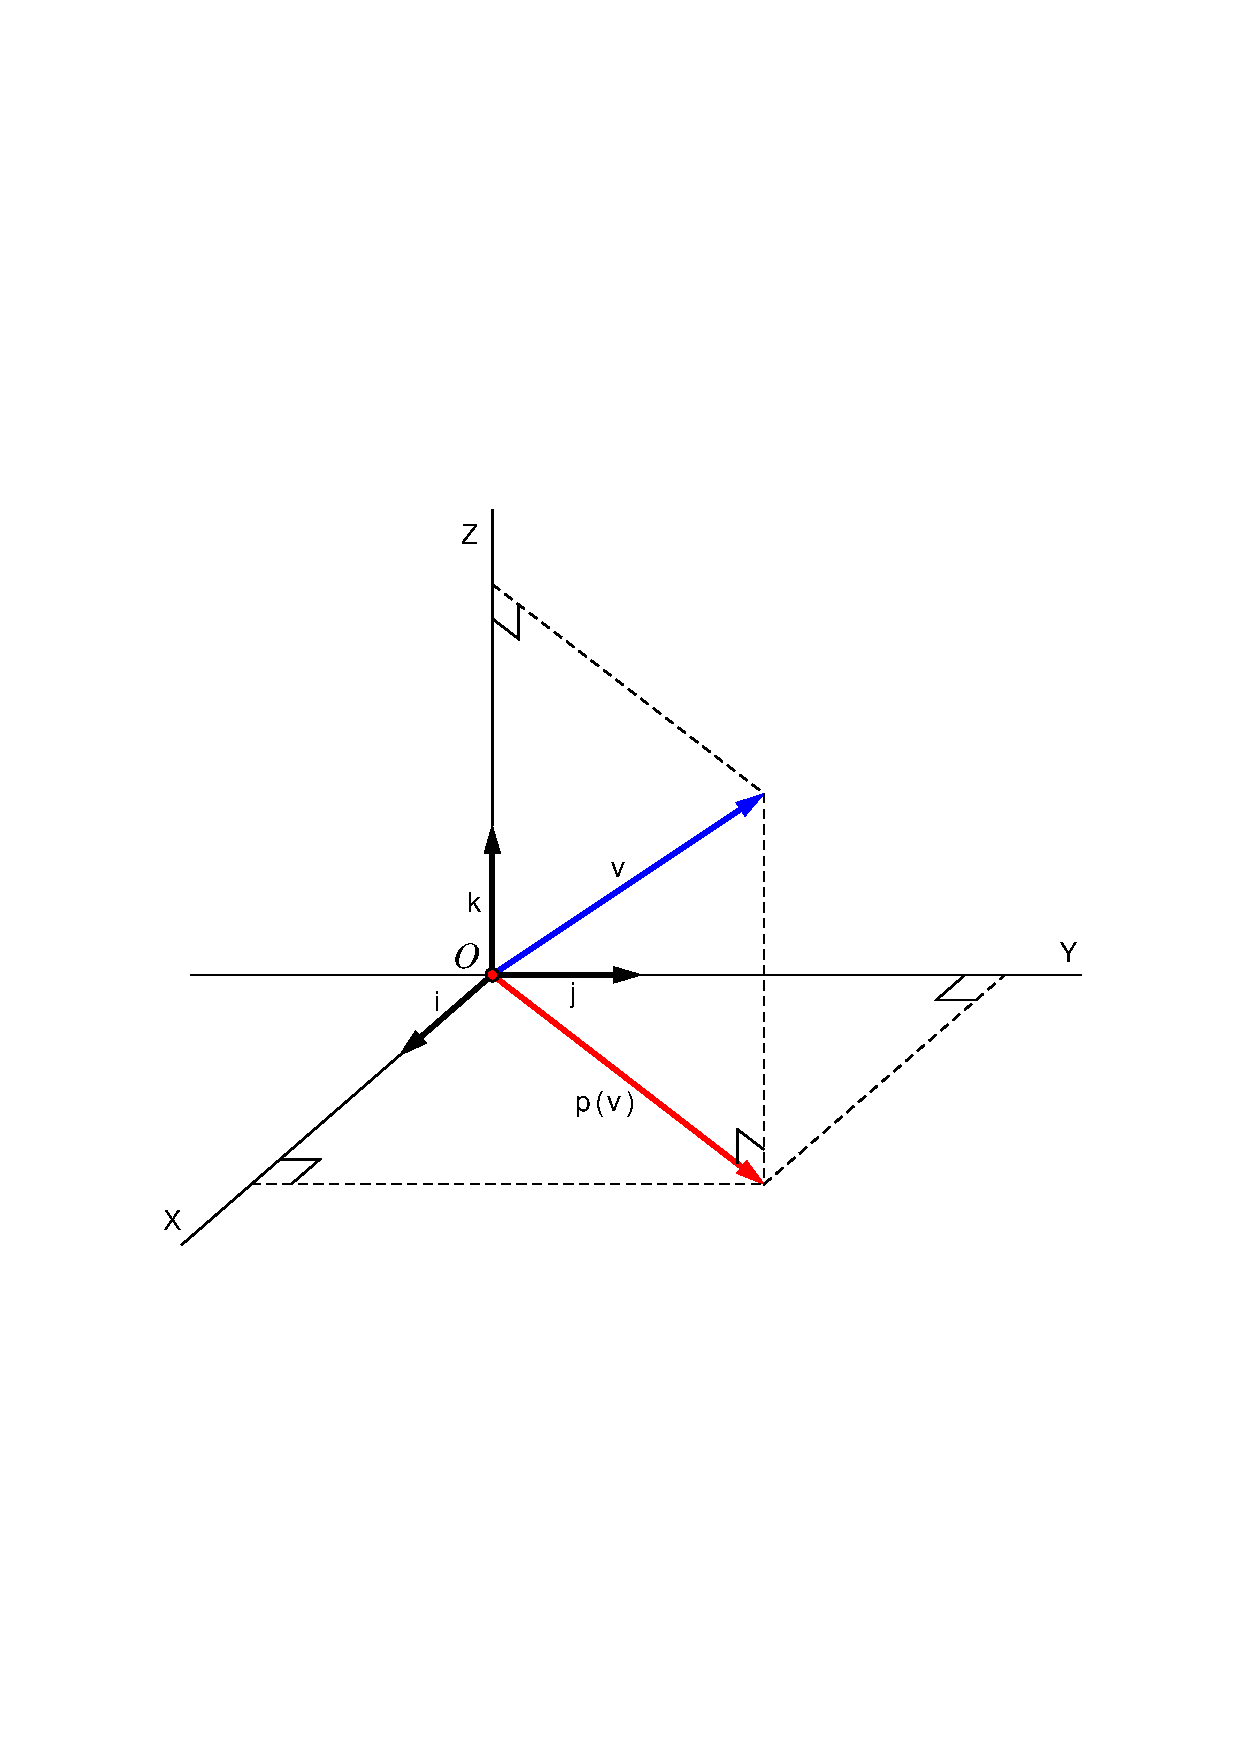
\includegraphics[trim=2cm 8cm 2cm
 8cm,width=0.50\textwidth,clip]{projektion.pdf}
  \\Figur 9.6: Egenværdiproblemet for projektion ned i  $(X,Y)$-planen.
\end{center}

Det er vist i \tref{NUID21-tn8.opgDimension2}{opgave}, at $\,p\,$ er lineær. Bestem samtlige egenværdier og de egenrum der hører til egenværdierne, udelukkende ved hovedregning (grubling).
\end{exercise}

\begin{example}[Egenværdiproblem for differentiation]\label{evExponential}
Vi betragter den lineære afbildning $f:C^{\infty}(\reel)\rightarrow C^{\infty}$ som er givet ved
$$
f(x(t))=x'(t)\,.
$$
Lad $\lambda$ være en vilkårlig skalar. Da der gælder
$$
f(\mathrm{e}^{\lambda t})=\lambda\,\mathrm{e}^{\lambda t}\,,
$$
er $\lambda$ en egenværdi for $f\,$, og $\mathrm e ^{\lambda t}$ er en egenvektor som hører til $\lambda\,$.\\

Da samtlige løsninger til differentialligningen
$$x'(t)=\lambda x(t)$$
er givet ved $\,k\cdot \mathrm{e}^{\lambda t}\,$, hvor $k$ er et vilkårligt reelt tal, er egenrummet hørende til $\lambda$ bestemt ved
$$E_{\lambda}= \maengde{k\cdot\e^{\lambda t} }{ k \in \reel}\,.$$
\end{example}

\subsection{Teoretiske pointer}

Den følgende hjælpesætning giver et vigtigt resultat for lineære afbildninger af vektorrum ind i sig selv. Den gælder uanset om det betragtede vektorrum har endelig dimension eller ej.

\begin{lemma}\label{th.evLinUafh}
Lad $\,f:V\rightarrow V$ være en lineær afbildning af et vektorrum $V$ ind i sig selv, og antag
\begin{enumerate}
\item
at $f$ har en række egenværdier med tilhørende egenrum,
\item
at der udvælges nogle af egenrummmene, og inden for hvert af de udvalgte egenrum udvælges nogle lineært uafhængige vektorer,
\item
og at alle de således udvalgte vektorer sættes sammen til ét vektorsæt $v\,$.
\end{enumerate}
Så er $\,v\,$ et lineært uafhængigt vektorsæt.
\end{lemma}

\begin{bevis}
Lad $\,f:V\rightarrow V$ være en lineær afbildning, og lad $v$ være et vektorsæt der er sammensat i overensstemmelese med punkt 1. til 3. i hjælpesætning \ref{th.evLinUafh}. Vi skal vise et $v$ er lineært uafhængigt. Den røde tråd i beviset er at vi antager det modsatte, det vil sige at $v$ er lineært afhængigt, og viser at dette fører til en modstrid.\\

Vi udtynder først $v$ til en basis for $ \Span\{v\} $. Der må da være mindst én vektor i $v$ som ikke er med i basen. Vi vælger en af slagsen, lad os kalde den $\mathbf x$. Nu skriver vi $\mathbf x$ som en linearkombination af basisvektorerne, idet vi  udelader de trivielle led, det vil sige dem som har koefficienten $0$:
\begin{equation}\label{uafhEgenvektorer}
\mathbf x=k_1\mv_1+\cdots+k_m\mv_m
\end{equation}
Vi kalder egenværdien der hører til $\mathbf x$ for $\lambda$, og egenværdierne hørende til $\mv_i$ for $\lambda_i$. Vi kan ud fra (\ref{uafhEgenvektorer}) opnå et udtryk for $\lambda\mathbf x$ på to forskellige måder, dels ved at gange (\ref{uafhEgenvektorer}) med  $\lambda$, dels ved at finde billedet ved $f$ af højre- og venstresiden i (\ref{uafhEgenvektorer}):
\begin{align*}
\lambda\mathbf x &=\lambda k_1\mv_1+\cdots+\lambda k_m\mv_m\\
\lambda\mathbf x &=\lambda_1 k_1\mv_1+\cdots+\lambda_m k_m\mv_m
\end{align*}
Ved subtraktion af den øverste ligning med den nederste medfører dette:
\begin{equation}\label{uafhEgenvektorer2}
\mnul=k_1(\lambda-\lambda_1)\mv_1+\cdots+k_m(\lambda-\lambda_m)\mv_m\,.
\end{equation}
Hvis alle koefficienterne til vektorerne på højresiden af (\ref{uafhEgenvektorer2}) er lig med nul, må $\lambda=\lambda_i$ for alle $i=1,2,\ldots, m$. Men så er $\mathbf x$ og alle basisvektorerne $\mv_i$ valgt fra det samme egenvektorrum, og de skulle derfor som samlet sæt være lineært uafhængige, sådan er de valgt. Dette strider mod at $\mathbf x$ er en linearkombination af basisvektorerne.\bs
Derfor må mindst én koefficienterne i (\ref{uafhEgenvektorer2}) være forskellig fra 0. Men så er nul-vektoren opskrevet som en egentlig linearkombination af basisvektorerne. Dette strider mod kravet om at en basis er lineært uafhængig.\bs
Konklusion: antagelsen om at $v$ er et lineært afhængigt vektorsæt, fører nødvendigvis til en modstrid. Derfor er $v$ lineært uafhængigt.
\end{bevis}

\begin{example}[Egenvektorers lineære uafhængighed]
En lineær afbildning $\,f:V\rightarrow V\,$ har tre egenværdier $\lambda_1, \lambda_2$ og $\lambda_3\,$ som har de geometriske multipliciteter $2$, henholdsvis $1$ og $3\,.$ Vektorsættet $(\ma_1,\ma_2)$ er en basis for $\,E_{\lambda_1}\,,$ $(\mb)$ er en basis for $\,E_{\lambda_2}\,,$ og $(\mc_1,\mc_2,\mc_3)$ er en basis for $\,E_{\lambda_3}\,.$ Så følger det af hjælpesætning \ref{th.evLinUafh} at ehvert udvalg af de seks basisvektorer er et lineært uafhængigt vektorsæt.
\end{example}

Værdien af hjælpesætning \ref{th.evLinUafh} viser sig ved at den direkte fører til de følgende vigtige resultater:

\begin{theorem}[Generelle egenskaber]\label{maxEvEn}
Lad $V$ være et vektorrum med dim$(V)\,$ = $n\,,$ og lad  $\,f:V\rightarrow V\,$ være en lineær afbildning af $V$ ind i sig selv. Der gælder:
\begin{enumerate}
\item
Egentlige egenvektorer som hører til forskellige egenværdier for $f\,,$ er lineært uafhængige.
\item
$f$ kan højst have $n$ forskellige egenværdier. 
\item
Hvis $f$ har $n$ forskellige egenværdier, findes der en basis for $\,V\,$ bestående af egenvektorer for $f\,$. 
\item
Summen af de geometriske multipliciteter af egenværdierne for $f$ kan højst være $n\,$.
\item
Hvis og kun hvis summen af de geometriske multipliciteter af egenværdierne for $f$ er lig med $n$, findes der en basis for $\,V\,$ bestående af egenvektorer for $f\,$.
\end{enumerate}
\end{theorem}

\begin{exercise}\label{EVegenskaber}
Det første punkt i sætning \ref{maxEvEn} er et simpelt specialtilfælde af hjælpesætning \ref{th.evLinUafh} og følger derfor umiddelbart af hjælpesætningen. Det andet punkt kan bevises således:\bs
\textit{Antag at en lineær afbildning har $k$ forskellige egenværdier. Vi vælger en egentlig vektor fra hvert af de $k$ egenrum. Sættet af de $k$ valgte vektorer er da i følge hjælpesætning \ref{th.evLinUafh} lineært uafhængigt, og $k$ må derfor være mindre end eller lig med vektorrummets dimension (se \tref{NUID18-fundLemma}{hjælpesætning})}.\bs
Gør på tilsvarende vis rede for hvordan de tre sidste punkter i sætning \ref{maxEvEn} følger af hjælpesætning \ref{th.evLinUafh}.
\end{exercise}

Motiveret af sætning \ref{maxEvEn} indfører vi begrebet egenbasis:
 
\begin{definition}[Egenvektorbasis]
Lad $\,f:V\rightarrow V$ være en lineær afbildning af et endeligt-dimensionalt vektorrum $V$ ind i sig selv.\bs
Ved en \textit{egenvektorbasis}, eller kort \textit{egenbasis}, for $V$ med hensyn til $f$ forstås en basis bestående af egenvektorer for $f\,$.
\end{definition}

Herefter kan vi præsenterer dette afsnits hovedresultat:

\begin{theorem}[Hovedsætning]\label{MainTh}
Lad $\,f:V\rightarrow V$ være en lineær afbildning af et $n$-dimensionalt vektorrum $V$ ind i sig selv, og lad $\,v=(\mv_1,\ldots\mv_n)\,$ være en basis for $V\,.$ Der gælder da:\bs 
1. Afbildningningsmatricen $\,\matind vFv\,$ for $f$ med hensyn til $v$ er en diagonalmatrix hvis og kun hvis $v$ er en egenbasis for $V$ med hensyn til $f\,$. \bs 
2. Antag at $v$ er en egenbasis $V$ med hensyn til $f\,,$ og $\,\mL\,$ betegne den diagonalmatrix som er afbildningsmatrix for $f$ med hensyn til $v\,.$ Rækkefølgen af diagonalelementerne i $\,\mL\,$ er da bestemt ud fra den valgte basis således: Basisvektoren $\,\mv_i\,$ hører til den egenværdi $\lambda_i$ som står i den $ i $'te søjle i $\,\mL\,$. 
\end{theorem}

Vi udskyder beviset for denne sætning til \tref{NUID24-tn10}{eNote} om diagonalisering.

\begin{example}[Diagonalmatrix for spejling]\label{spejling2}
Lad os igen betragte situationen i eksempel \ref{spejling}, hvor vi betragtede afbildningen $\,s\,$ som spejler vektorer afsat ud fra Origo i linjen $\,m\,$:
\begin{center}
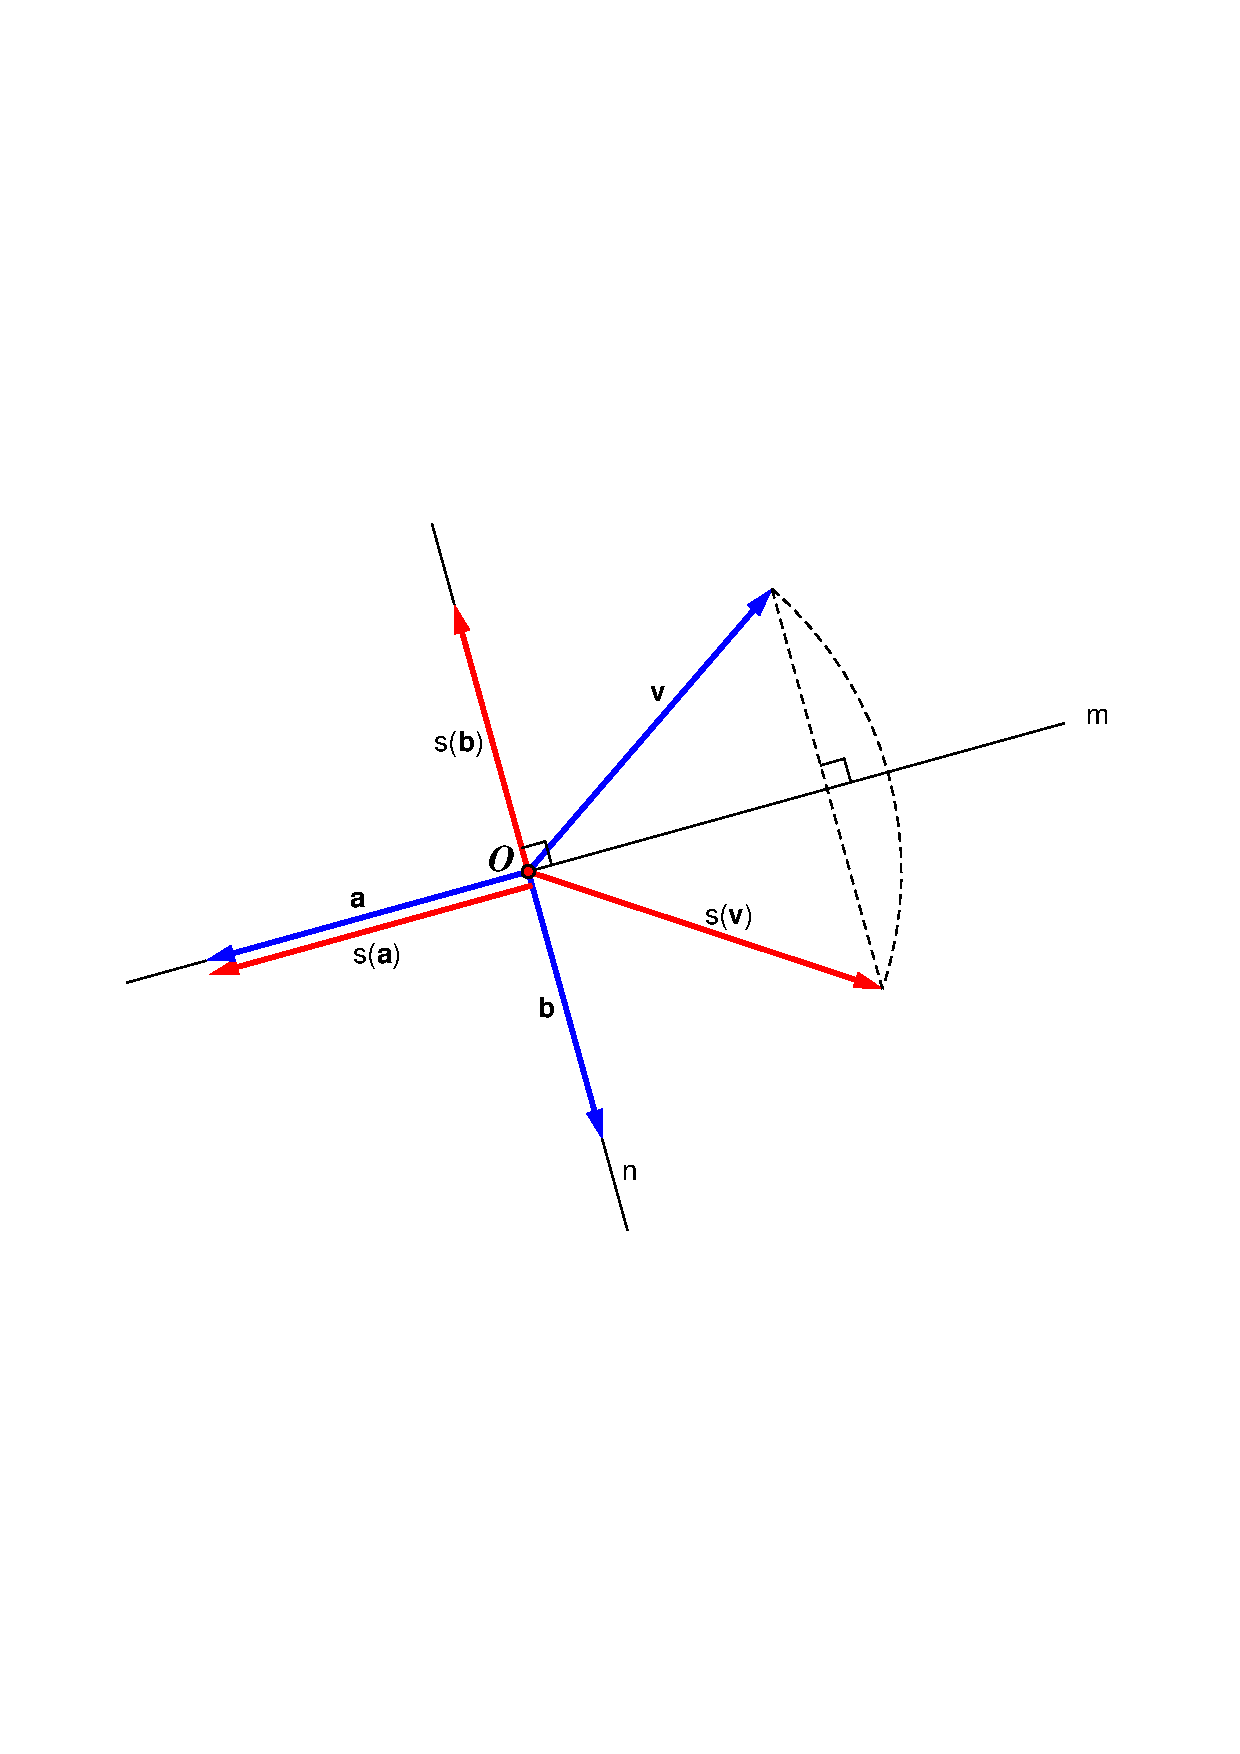
\includegraphics[trim=2cm 9.2cm 2cm 9cm,width=0.6\textwidth,clip]{evSpejling.pdf}  
\end{center}
Vi fandt at $\,\ma\,$ er en egenvektor som hører til egenværdien $\,1\,$, og at $\,\mb\,$ er en egenvektor som hører til egenværdien $\,-1\,$. Da planen har dimensionen 2 følger det af sætning \ref{MainTh} at hvis vi vælger basen $\,(\ma,\mb)\,$, så har $f$ den følgende afbildningsmatrix med hensyn til denne basis:
$$\begin{matr}{rr}1&0\\0&-1\end{matr}\,.$$
\end{example}

\begin{example}[Lineær afbildning uden egenværdier]
I eksempel \ref{hatvektor} fandt vi at afbildningen ``tværvektor'' i $(G_2,\reel)$ ingen egenværdier har. Der findes derfor ingen egenbasis for afbildningen, og den kan derfor ikke beskrives ved en diagonalmatrix for denne afbildning.
\end{example}

\begin{example}[Diagonalisering af kompleks afbildning]
Lad $f:\mathbb C^2 \rightarrow \mathbb C^2$ være en lineær afbildning som opfylder
\begin{equation*}f(z_1,z_2)=(-z_2,z_1)\,.\end{equation*}
Da der gælder:
$$ f(i,1)=(-1,i)=i\,(i,1)\quad \mathrm{og} \quad f(-i,1)=(-1,-i)=(- i)(-i,1)\,,$$
ses at $i$ er en egenværdi for $f$ med en tilhørende egenvektor $(i,1)$, og at $-i$ er en egenværdi for $f$ med en tilhørende egenvektor $(-i,1)\,.$\bs
Da $(i,1)$ og $(-i,1)$ er lineært uafhængige, er $\big(\,(i,1),(-i,1)\,\big)$ en egenbasis for $\mathbb C^2$ med hensyn til $f\,.$ Afbildningsmatricen for $f$ med hensyn til denne basis er i følge sætning \ref{MainTh}
\begin{equation*}\begin{matr}{rr}i&0\\0&-i\end{matr}\,.\end{equation*}
\end{example}

\begin{exercise}\label{evProjektion2}
Betragt igen situationen i eksempel \ref{evProjektion}. Vælg to forskellige egenbaser (baser bestående af egenvektorer for $\,p\,$), og bestem i hvert af de to tilfælde den diagonalmatrix som bliver afbildningsmatrix for $\,p\,$ med hensyn til den valgte basis. 
\end{exercise}

%
\end{document} 
%\begin{bevis}

%Antag at summen af de geometriske multipliciteter er større end $n\,$. Vi vælger da det antal lineært uafhængige vektorer i hvert af egenrummene som svarer til egenrummet dimension. Det samlede sæt vil da ifølge sætning \ref{th.evLinUafh} indholde flere end $n$ lineært uafhængige vektorer. Det er umuligt, derfor er antagelsen falsk.\bs
%Antag at summen af de geometriske multipliciteter er lig med $n\,$. Vi vælger da det antal lineært uafhængige vektorer i hvert af egenrummene som svarer til egenrummet dimension. Det samlede sæt vil da indeholde $n$ lineæart uafhænigige egenvektorer for $f$ som kan vælges som basis for $V$.
%\end{bevis}



\section{Egenværdiproblemet for kvadratiske matricer}

Når en lineær afbildning $\,f:V\rightarrow V\,$ afbilder et $n$-dimensionalt vektorrum $V$ ind i vektorrummet selv, bliver afbildningsmatricen for $f$ med hensyn til en vilkårligt valgt  basis $a$ en \textit{kvadratisk} matrix. Egenværdiproblemet $f(\mv)=\lambda \mv$ er da ækvivalent med matrixligningen:
\begin{equation}\label{EvForAfbmatrix}
\matind aFa \mathbf{\cdot} \vekind av=\lambda \cdot \vekind av\,.\end{equation}
Dette giver os anledning til formulere et egenværdiproblem for kvadratiske matricer generelt, det vil sige uden at vi nødvendigvis behøver at tænke på den kvadratiske matrix som en afbildningsmatrix. Vi vil opstille  stanar\-diserede måder at gå frem på, når man egenværdier og egenvektorer for kvadratiske matricer søges bestemt. Dermed fås samtidigt, i kraft af (\ref{EvForAfbmatrix}), metoder til at finde egenværdier og egenvektorer for alle lineære afbilninger af vektorrum ind i sig, der kan beskrives ved hjælp af afbildningsmatricer.\\
 
Først præciserer vi hvad der forstås ved egenværdiproblemet for en kvadratisk matrix.

\begin{definition}[Egenværdiproblemet for matricer] \label{def.eig}
At løse egenværdiproblemet for en kvadratisk reel $n \times n$-matrix $\,\mA\,$ vil sige at finde en skalar $ \lambda $ og en egentligt vektor $\mv=(v_1,\,...\,,v_n)$ som opfylder ligningen:
\begin{equation}\label{def.eig.formel1}
\mA \,\mv = \lambda \mv \,.
\end{equation}\
Opfyldes denne ligning for et par af $ \lambda $ og $ \mv \neq \mathbf 0 $, kaldes $ \lambda $ for en \textit{egenværdi} for $\mA$ og $\mv $ en til $\lambda$ hørende \textit{egenvektor} for $\mA\,.$ 
\end{definition}

\begin{example}[Egenværdiproblem for kvadratisk matrix]
Det ønskes undersøgt om $ \mv_1 = (2,3) $, $ \mv_2 = (4,4) $ og $ \mv_3 = (2,-1) $ er egenvektorer for $ \mA $ givet ved
\begin{equation}
\mA = \begin{matr}{rr} 4 & -2 \\ 3 & -1 \end{matr}
\end{equation}
Til dette opstilles egenværdiproblemet, som beskrevet i definition \ref{def.eig}.
\begin{equation}
\begin{aligned}
\mA\mv_1 &= \begin{matr}{rr} 4 & -2 \\ 3 & -1 \end{matr} \begin{matr}{r} 2 \\ 3 \end{matr} = \begin{matr}{r} 2 \\ 3 \end{matr} = 1 \cdot \mv_1 \\
\mA\mv_2 &= \begin{matr}{rr} 4 & -2 \\ 3 & -1 \end{matr} \begin{matr}{r} 4 \\ 4 \end{matr} = \begin{matr}{r} 8 \\ 8 \end{matr} = 2 \cdot \mv_2 \\
\mA\mv_3 &= \begin{matr}{rr} 4 & -2 \\ 3 & -1 \end{matr} \begin{matr}{r} 2 \\ -1 \end{matr} = \begin{matr}{r} 10 \\ 7 \end{matr} \neq \lambda \cdot \mv_3 \,.
\end{aligned}
\end{equation}
Af dette ses at $ \mv_1 $ og $ \mv_2 $ er egenvektorer for $ \mA $. $ \mv_1 $ hører til egenværdien 1, og $ \mv_2 $ hører til egenværdien 2. \bs
Endvidere ses at $ \mv_3 $ ikke er en en egenvektor for $ \mA $.
\end{example}

\begin{example}[Egenværdiproblem for kvadratisk matrix]
Givet matricen
\begin{equation*}\mA=\begin{matr}{rr}2&-2\\-2&-3\end{matr}\,.\end{equation*}
Da
\begin{equation*}\mA=\begin{matr}{rr}2&-2\\-2&2\end{matr}\,
\begin{matr}{r}1\\1\end{matr}
=\begin{matr}{r}0\\0\end{matr}
=0\,\begin{matr}{r}1\\1\end{matr}\,,
\end{equation*}
er $0$ en egenværdi for $\mA$ og $(1,1)$ er en til $0$ hørende egenvektor for $\mA\,.$
\end{example}

\begin{example}[Egenværdiproblem for kvadratisk matrix]
Givet matricen
\begin{equation*}\mA=\begin{matr}{rr}0&1\\-1&0\end{matr}\,.\end{equation*}
Da
\begin{equation*}\mA=\begin{matr}{rr}0&1\\-1&0\end{matr}\,
\begin{matr}{r}-i\\1\end{matr}
=\begin{matr}{r}1\\i\end{matr}
=i\,\begin{matr}{r}-i\\1\end{matr}\,,
\end{equation*}
er $i$ en kompleks egenværdi for $\mA$ og $(-i,1)$ er en til $i$ hørende kompleks egenvektor for $\mA\,.$
\end{example}

Til brug for de følgende undersøgelser knytter vi nogle vigtige kommentarer til definition \ref{def.eig} .\bs
Først bemærker vi at selv om den kvadratiske matrix $\mA$ i definition \ref{def.eig} er reel, er man ofte interesseret i ikke kun at finde reelle løsninger til ligningen (\ref{def.eig.formel1}), men generelt komplekse løsninger. Der søges med andre ord en skalar $\lambda \in \mathbb C$ og en vektor $\mv \in \mathbb C^n\,,$ der opfylder (\ref{def.eig.formel1}). \bs
Det kan derfor være hensigtsmæssigt at opfatte venstresiden i (\ref{def.eig.formel1}) som en afbildning $\,f:\mathbb C^n \rightarrow \mathbb C^n\,$ givet ved:
\begin{equation*}
f(\mv)=\mA\,\mv\,.
\end{equation*}
Denne afbildning er lineær. Lad nemlig $\mathbf u\in \mathbb C^n\,$, $\mathbf v\in \mathbb C^n\,$ og $k\in \mathbb C\,.$ Der gælder da ifølge sædvanlige regneregler for matricer 
\begin{equation*}
\begin{aligned}
1.\quad f(\mathbf u + \mv)&=\mA\,(\mathbf u+\mv)=\mA\,\mathbf u +\mA\,\mv\\
2. \quad f(k\,\mathbf u)&=\mA(k\,\mathbf u)=k(\mA\,\mathbf u)
\end{aligned}
\end{equation*}
Hermed er lineariteten vist. Da egenværdiproblemet $\,f(\mv)=\lambda \mv\,$ i dette tilfælde er \textit{identisk} med egenværdiproblemet $\,\mA \mv=\lambda \mv\,$, kan det sluttes at resultaterne opnået i afsnit $9.1$ for egenværdiproblemet i almindelighed, umiddelbart kan overføres til egenværdiproblemet for matricer. Lad os således straks karakterisere mængden af egenvektorer der hører til en given egenværdi for en kvadratisk, reel matrix, sammenlign med sætning \ref{thLambdaUrum}.

\begin{theorem}[Underrum af egenvektorer] \label{saet.egenrum}
Lad $ \lambda $ være en reel eller kompleks egenværdi for en reel  $n\times n$-matrix  $ \mA $. Der gælder da at mængden af komplekse egenvektorer for $ \mA $ hørende til $ \lambda $, er et underrum i $\mathbb C^n$. 
\end{theorem}

Hvis man kun er interesseret i reelle løsninger på egenværdiproblemet for reelle kvadratiske matricer, kan man alternativt opfatte venstresiden i (\ref{def.eig.formel1}) som en reel afbildning $\,f:\mathbb R^n \rightarrow \mathbb R^n\,$ givet ved:
\begin{equation*}
f(\mv)=\mA\,\mv\,.
\end{equation*}
Denne afbildning er naturligvis også lineær. Vi opnår herved følgende variant af sætning \ref{saet.egenrum}:

\begin{theorem} [Underrum af egenvektorer]\label{saet.egenrum.reel}
Lad $ \lambda $ være en reel egenværdi for en reel  $n\times n$-matrix  $ \mA $. Der gælder da at mængden af reelle egenvektorer for $ \mA $ hørende til $ \lambda $, er et underrum i $\mathbb R^n$. 
\end{theorem}

I lyset af sætning \ref{saet.egenrum.reel} og sætning \ref{saet.egenrum.reel} indfører vi begrebet egenvektorrum, sammenlign med definition \ref{defErum}.

\begin{definition}[Egenvektorrum]
Lad $\mA$ være en kvadratisk, reel matrix, og lad $\lambda$ være en egenværdi for $\mA\,.$\bs
Underrummet af alle de til $\lambda$ hørende egenvektorer kaldes \ind{egenvektorrum}{egenvektorrummet} (eller kort \ind{egenrum}{egenrummet}) hørende til $\lambda$ og betegnes $ E_\lambda\,. $
\end{definition}

Efter at vi nu har opridset de grundlæggende strukturelle rammer for egenværdiproblemet for kvadratiske matricer, vil vi i de to følgende delafsnit helt elementært undersøge, hvordan man overhovedet kan gå i gang med at finde egenværdier og egenvektorer for kvadratiske matricer.\bs
%\begin{theorem}
%Lad $\mA$ være en reel $n\times n$, og lad $\lambda$ være en reel eller kompleks egenværdi for $\mA\,.$ Der gælder da at mængden af mængden af egenvektorer som hører til $\lambda\,,$ et underrum i $\mathbb C^n\,.$
%\end{theorem}
\subsection{At finde egenværdierne for en kvadratisk matrix}

Vi ønsker at bestemme de egenværdier, som hører til en reel $n\times n$ matrix $\mA\,$. Udgangspunktet er som nævnt ligningen
\begin{equation}
\mA \mv = \lambda \mv \,,
\end{equation}

I første omgang sætter vi $\lambda \mv$ over på venstresiden af lighedstegnet, hvorefter $ \mv $ ``tages uden for parentes''. Det kan gøres fordi $\, \mv = \mE\, \mv \,$ hvor $\,\mE\,$ er enhedsmatricen:
\begin{equation} \label{lig.omskrivning}
\mA \mv = \lambda \mv \; \Leftrightarrow \; \mA \mv - \lambda \mE \mv = \mnul \; \Leftrightarrow \; (\mA - \lambda \mE) \mv = \mnul \,. 
\end{equation}
Den sidste ligning i (\ref{lig.omskrivning}) svarer til et homogent lineært ligningssystem bestående af $n$ ligninger med de $n$ ubekendte $v_1,\,...,\,v_n$, som er elementerne i $\mv=(v_1,\,...,\,v_n)\,.$ Det er dog ikke muligt straks at løse ligningssystemet, netop fordi vi ikke kender $ \lambda $. Vi er nødt til at arbejde videre med ligningssystemets koefficientmatrix, som tildeles et særligt symbol: $$ \mathbf K_\mA(\lambda) = (\mA - \lambda \mE) $$ og kaldes \ind{den karakteristiske matrix}{den karakteristiske matrix} for $ \mA $. \bs
Da det er et homogent lineært ligningssystem, som skal løses, er der som udgangspunkt to muligheder for løsningsstrukturen. Enten er den karakteristiske matrix \textit{regulær}, og så er den eneste løsning $ \mv=\mnul\, $. Eller også er matricen \textit{singulær}, og der vil findes uendeligt mange løsninger $ \mv $. Men da definition \ref{def.eig} kræver at $ \mv $ skal være en egentlig vektor, altså en vektor forskellig for nulvektoren, må den karakteristiske matrix være singulær. For at undersøge om dette gælder, tages determinanten af den karakteristiske matrix. Den er nul netop når matricen er singulær:
\begin{equation}\label{detLign}
\det(\mA - \lambda \mE) = 0\,.
\end{equation}
Bemærk at venstresiden i \eqref{detLign} er et polynomium med $\lambda$ som variabel. Polynomiet tildeles et særligt symbol:
$$ K_\mA(\lambda) = \det(\mA - \lambda \mE) = \det(\mK_\mA (\lambda) )$$ 
og kaldes \ind{det karakteristiske polynomium}{det karakteristiske polynomium} for $ \mA \,.$ \bs
Den ligning der fremkommer når det karakteristiske polynomium sættes lig nul
$$ K_\mA(\lambda) = \det(\mA - \lambda \mE) = \det(\mK_\mA (\lambda) )=0$$ 
kaldes \ind{karakterligningen}{karakterligningen} for $ \mA $. \bs 
Ved hjælp af udregningsmetoden for determinant kan det indses at det karakteristiske polynomium altid er et $n$'te gradspolynomium. Se også de efterfølgende eksempler. Hovedpointen er at rødderne i det karakteristiske polynomium (løsningerne til karakterligningen) er egenværdierne for matricen, fordi egenværdierne netop opfylder, at den karakteristiske matrix er singulær.

\begin{example}[Egenværdier for $2\times 2$ matricer] \label{eks.eigvaer}
Givet to matricer $ \mA $ og $ \mB $:
\begin{equation}
\mA = \begin{matr}{rr} 4 & -2 \\ 3 & -1 \end{matr} \quad \textrm{og} \quad \mB = \begin{matr}{rr} -1 & 4 \\ -2 & 3 \end{matr}\,.
\end{equation}
Vi ønsker at bestemme egenværdierne for $ \mA $ og $ \mB $. \bs
Først betragtes $ \mA $. Dens karakteristiske matrix opskrives:
\begin{equation}
\mathbf K_\mA(\lambda) = \mA - \lambda\mE = \begin{matr}{rr} 4 & -2 \\ 3 & -1 \end{matr} - \begin{matr}{cc} \lambda & 0 \\ 0 & \lambda \end{matr} = 
\begin{matr}{cc} 4-\lambda & -2 \\ 3 & -1-\lambda \end{matr}\,.
\end{equation}
Nu bestemmes det karakteristiske polynomium:
\begin{equation}
\begin{aligned}
K_\mA(\lambda) &= \det(\mathbf K_\mA(\lambda)) = \det\!\left(\begin{matr}{cc} 4-\lambda & -2 \\ 3 & -1-\lambda \end{matr} \right) \\
&= (4-\lambda)(-1-\lambda) - (-2) \cdot 3 = \lambda^2 - 3\lambda + 2 \,.
\end{aligned}
\end{equation}
Polynomiet har som forventet graden $2\,$. Karakterligningen kan opskrives og løsningerne til den kan bestemmes:
\begin{equation}
K_\mA(\lambda) = 0 \; \Leftrightarrow \; \lambda^2 - 3\lambda + 2 = 0 \; \Leftrightarrow \; \lambda = 1 \,\,\,\mathrm{eller} \,\,\,\lambda = 2 \,.
\end{equation}
Altså har $ \mA $ to egenværdier: $\lambda_1=1$ og $\lambda_1=2\,$.\bs
Den samme teknik bruges for at bestemme eventuelle egenværdier til $ \mB $.
\begin{equation}
\begin{aligned}
\mathbf K_\mB(\lambda) &= \mB - \lambda\mE = \begin{matr}{rr} -1 & 4 \\ -2 & 3 \end{matr} - \begin{matr}{cc} \lambda & 0 \\ 0 & \lambda \end{matr} = 
\begin{matr}{cc} -1-\lambda & 4 \\ -2 & 3-\lambda \end{matr} \\
K_\mB(\lambda) &= \det(\mK_\mB(\lambda)) = \det\!\left(\begin{matr}{cc} -1-\lambda & 4 \\ -2 & 3-\lambda \end{matr} \right) \\
&= (-1-\lambda)(3-\lambda) - 4 \cdot (-2) = \lambda^2 - 2\lambda + 5 \,.
\end{aligned}
\end{equation}
Der er i dette tilfælde ingen reelle løsninger til $ K_\mB(\lambda) = 0 $, fordi diskriminanten $ d = (-2)^2- 4 \cdot 1 \cdot 5 = -16 < 0 $, og derfor har $ \mB $ ingen reelle egenværdier. Men den har to komplekse egenværdier. Vi tager den komplekse ``værktøjskasse'' frem:   Diskriminanten kan omkrives til $ d = (4i)^2 $, hvilket giver de to komplekse løsninger 
\begin{equation}
\lambda = \frac{2 \pm 4i}{2} \; \Leftrightarrow \; \lambda = 1 + 2i \; \textrm{ og } \; \bar{\lambda} = 1-2i
\end{equation}
Altså har $ \mB $ to komplekse egenværdier: $\lambda_1=1+2i$ og $\lambda_2=1-2i\,$.\bs 
\end{example}

%Som det fremgår af eksempel \ref{eks.eigvaer}, er det ikke altid at der findes reelle løsninger til karakterligningen, og derfor heller ingen egenværdier til matricen. Ligeså kunne man forestille sig, at der kun findes ``få'' reelle egenværdier matricens størrelse taget i betragtning. Antallet af reelle egenværdier til en matrix er derfor ikke entydigt bestemt af dens størrelse. I afsnit \ref{sek.kompl} tages egenværdiproblemet op i kompleks sammenhæng, hvor det altid vil være muligt at bestemme egenværdier til en matrix.\bs

I den følgende sætning opsummeres konklusionerne i dette delafsnit.

\begin{theorem}[Det karakteristiske polynomium]\label{karakteristiskP}
For den kvadratiske reelle $n \times n$-matrix $\,\mA\,$ betragtes 
\begin{enumerate}
\item \textit{Den karakteristiske matrix} $ \mathbf K_\mA(\lambda) = \mA - \lambda \mE \,.$
\item \textit{Det karakteristiske polynomium} $ K_\mA(\lambda) = \det(\mK_\mA(\lambda)) = \det(\mA - \lambda \mE)\,. $
\item \textit{Karakterligningen} $ K_\mA(\lambda) = 0\,.$
\end{enumerate}

Der gælder:\bs
1. Det karateristiske polynoium er et $n$'te gradspolynomium med den variable $\lambda\,$, og karakterligningen er tilsvarende en $n$'te gradsligning med den ubekendte $\lambda\,.$\bs
2. Rødderne i det karakteristiske polynomium (løsningerne for karakterligningen) er samtlige egenværdier for $ \mA\,.$
\end{theorem}

\subsection{At finde egenvektorerne for en kvadratisk matrix}

Efter at egenværdierne til en reel $n\times n$ matrix $\mA$ er bestemt, er det muligt at bestemme de tilhørende egenvektorer. Proceduren tager udgangspunkt i ligningen
\begin{equation}\label{omskrivn}
(\mA - \lambda \mE) \mv = \mnul \,,
\end{equation}
som vi nåede frem til i \eqref{lig.omskrivning}. Da egenværdierne nu er kendte, kan det til (\ref{omskrivn}) svarende homogene lineære ligningssystem løses med hensyn til $n$ ubekendte $v_1,\,...,\,v_n$ som er elementerne i $\mv=(v_1,\,...,\,v_n)\,.$ Vi skal blot indsætte  egenværdierne efter tur. Som allerede nævnt er den karakteristiske matrix singulær, når den indsatte $ \lambda $ er en egenværdi. Derfor findes der uendeligt mange løsninger til ligningssystemet. At finde disse svarer til at finde samtlige egenvektorer $\mv$ der hører til $\lambda\,.$\bs 
I den følgende metode sammenfattes opgaven med at bestemme egenværdier og tilhørende egenvektorer for en kvadratisk matrix.

\begin{method}[Bestemmelse af egenvektorer] \label{met.eg}
Samtlige (reelle eller komplekse) egenværdier $ \lambda $ for den kvadratiske matrix $ \mA $ findes som løsningerne til \ind{karakterligning}{karakterligningen} for $ \mA $:
\begin{equation}
K_\mA(\lambda) = 0 \; \Leftrightarrow \; \det(\mA - \lambda \mE) = 0 \, .
\end{equation}
Derefter kan egenvektorerne $ \mv $ tilhørende hver enkelt egenværdi $ \lambda $ bestemmes. De er løsningerne til det følgende lineære ligningssystem
\begin{equation}
(\mA - \lambda \mE) \mv =  \mnul \,,
\end{equation}
når egenværdien $\lambda$ er indsat. $ \mE $ er enhedsmatricen.
\end{method}

Metode \ref{met.eg} udfoldes i de følgende tre eksempler, der også giver os anledning til, i forlængelse af sætning \ref{saet.egenrum} og sætning \ref{saet.egenrum.reel}, at karakterisere mængden af egenvektorer der tilhører en given egenværdi.
%\begin{obs}
%Læg mærke til at antallet af egenvektorer tilhørende en egenværdi ikke er fastsat i metode \ref{met.eg}. Der står kun, at hvis $ \mv $ er løsning til ligningssystemet $ (\mA - \lambda \mE) \mv =  \mnul $, så er den en egenvektor tilhørende egenværdien $ \lambda $. Det forklares yderligere i afsnit \ref{af.multi}.
%\end{obs}
%\begin{bevis}
%Vi ønsker i første omgang at bestemme en egenværdi til $ \mA $ og tager udgangspunkt i ligningen
%\begin{equation}
%\mA \mv = \lambda \mv \,.
%\end{equation}
%Der foretages en omskrivning:
%\begin{equation} \label{lig.beveg}
%\mA \mv = \lambda \mv \; \Leftrightarrow \; \mA \mv - \lambda \mv = \mnul \; \Leftrightarrow \; (\mA - \lambda \mE) \mv = \mnul \, .
%\end{equation}
%Det sidste udtryk vil altid gælde, hvis $ \mv = \mnul $. Det er imidlertid ikke nogen interessant løsning, og af samme grund skal egenvektorer altid være egentlige, jævnfør definition \ref{def.eig}. Da $ \mv $ er egentlig, må matricen $ (\mA - \lambda \mE) $ være singulær, fordi højresiden er nulvektoren. Determinanten af en singulær matrix er nul, hvorfor man kan bestemme samtlige egenværdier ved at løse ligningen
%\begin{equation}
%\det(\mA - \lambda \mE) = 0 \, .
%\end{equation}
%Når $ \lambda $ er bestemt indsættes det i udtrykket længst til højre i ligningerne \eqref{lig.beveg} for at finde tilhørende egenvektorer $ \mv $.
%\end{bevis}


\begin{example}[Egenværdiers tilhørende egenvektorer] \label{eks.1}
Givet den kvadratiske matrix
\begin{equation}
\mA = \begin{matr}{rr} 2 & 1 \\ 1 & 2 \end{matr}\,.
\end{equation}
Vi ønsker at bestemme egenværdier og egenvektorer til $ \mA $ og bruger metode \ref{met.eg}. Først findes den karakteristiske matrix:
\begin{equation}
\mK_\mA(\lambda) = \mA - \lambda \mE = \begin{matr}{rr} 2 & 1 \\ 1 & 2 \end{matr} - \begin{matr}{rr} \lambda & 0 \\ 0 & \lambda \end{matr} = \begin{matr}{cc} 2-\lambda & 1 \\ 1 & 2-\lambda \end{matr}
\end{equation}
Dernæst opstilles det karakteristiske polynomium:
\begin{equation}
\begin{aligned}
K_\mA(\lambda) &= 
\det(\mA - \lambda \mE) \\
=\det\! \left( \begin{matr}{cc} 2-\lambda & 1 \\
 1 & 2-\lambda \end{matr} \right)
 &= (2-\lambda)(2-\lambda) - 1\cdot 1 = \lambda^2 - 4 \lambda + 3\,.
\end{aligned}
\end{equation}
Karakterligningen, som er $ \lambda^2 - 4 \lambda + 3 = 0 $, har løsningerne $ \lambda_1 = 1 $ og $ \lambda_2 = 3 $, der er samtlige reelle egenværdier til $ \mA $. \bs
For at bestemme de til $ \lambda_1 $ hørende egenvektorer indsættes $ \lambda_1 $ i $ (\mA - \lambda \mE) \mv = \mnul $, hvorefter vi løser det hertil svarende lineære ligningssystem som har totalmatricen:
\begin{equation}
\mathbf T=\left[\mA - \lambda_1 \mE\,|\, \mnul\,\right]=\begin{matr}{cc|c} 2-1 & 1 & 0 \\ 1 & 2-1 & 0 \end{matr}\,.
\end{equation}
Ved GaussJordan-elimination fås
\begin{equation}
\mathrm{trap}(\mathbf T)=\begin{matr}{cc|c} 1 & 1 & 0 \\ 0 & 0 & 0 \end{matr}
\end{equation}
Der er altså uendeligt mange løsninger $ \mv = (v_1, v_2) $, da der kun er én ikke-triviel ligning: $ v_1 + v_2 = 0 $. Ønsker man blot én egentlig egenvektor tilhørende egenværdien $ \lambda_1 $, kan $ v_2 $ sættes til 1, og man får egenvektoren $ \mv_1 = (-1,1)\,. $ Samtlige reelle egenvektorer hørende til $ \lambda_1 $ kan da opskrives som
\begin{equation}
\mv=t\cdot \begin{matr}{r}-1\\1\end{matr}\,\,,\,t\in \reel\,.
\end{equation}
Dette er et én-dimensionalt underrum i $ \reel^2 $, nemlig egenrummet som hører til egenværdien $1\,$ som vi også kan angive således:
\begin{equation}
E_1=\Span\{(-1,1)\}\,.
\end{equation}

Nu indsættes $ \lambda_2 $ i $(\mA - \lambda \mE) \mv = \mnul $, hvorefter vi løser det hertil svarende lineære ligningssystem som har totalmatricen
\begin{equation}
\mathbf T=\left[\mA - \lambda_2 \mE\,|\, \mnul\,\right]=\begin{matr}{cc|c} 2-3 & 1 & 0 \\ 1 & 2-3 & 0 \end{matr}\,.
\end{equation}
Ved GaussJordan-elimination fås
\begin{equation}
\mathrm{trap}(\mathbf T)=\begin{matr}{cc|c} 1 & -1 & 0 \\ 0 & 0 & 0 \end{matr}\,.
\end{equation}

Heraf ses at $ \mv_2 = (1,1) $ er en egenvektor tilhørende egenværdien $ \lambda_2 $. Samtlige reelle egenvektorer hørende til $ \lambda_2 $ kan  opskrives som
\begin{equation}
\mv=t\cdot \begin{matr}{r}1\\1\end{matr}\,\,,\,t\in \reel\,.
\end{equation}
Dette er et én-dimensionalt underrum i $ \reel^2 $ som vi også kan angive ved:
\begin{equation}
E_3=\Span\{(1,1)\}\,.
\end{equation}
Der vil nu blive ført kontrol: Når $ \mv_1=(-1,1) $ afbildes med $ \mA $, vil billedvektoren da udelukkende være en skalering (længdeændring) af $ \mv_1 $?
\begin{equation}
\mA \mv_1 = \begin{matr}{rr} 2 & 1 \\ 1 & 2 \end{matr} \begin{matr}{r} -1 \\ 1 \end{matr} =  \begin{matr}{rr} -1 \\ 1 \end{matr} = \mv_1 \, .
\end{equation}
Det passer! Man kan oven i købet se, at egenværdien er $1\,$. \bs
Nu kontrolleres $ \mv_2 $:
\begin{equation}
\mA \mv_2 = \begin{matr}{rr} 2 & 1 \\ 1 & 2 \end{matr} \begin{matr}{r} 1 \\ 1 \end{matr} =  \begin{matr}{rr} 3 \\ 3 \end{matr} = 3 \cdot \mv_2 \, .
\end{equation}
$ \mv_2 $ er altså som forventet også en egenvektor, og egenværdien er 3.
\end{example}

\begin{example}[Komplekse egenværdier og egenvektorer]\label{komplexex}
I eksempel \ref{eks.eigvaer} er der givet en matrix $ \mB $ med
\begin{equation}
\mB = \begin{matr}{rr} -1 & 4 \\ -2 & 3 \end{matr}
\end{equation}
som ingen reelle egenværdier har. Men vi fandt to komplekse egenværdier, $\lambda_1=1+2i$ og $\lambda_2=1-2i\,.$\bs
Vi indsættes $\lambda_1$ i 
$ (\mB - \lambda \mE) \mv = \mnul $, hvorefter vi løser det hertil svarende lineære ligningssystem som har totalmatricen
\begin{equation}
\mathbf T=\left[\mB - \lambda_1 \mE\,|\, \mnul\,\right]=
\begin{matr}{cc|c} -1-(1+2i) & 4 & 0\\ -2 & 3-(1+2i) & 0 \end{matr}
\end{equation}
Ved GaussJordan-elimination fås  
\begin{equation}
\mathrm{trap}(\mathbf T)=
\begin{matr}{cc|c} 1 & -1+i & 0 \\ 0 & 0 & 0 \end{matr}
\end{equation}

Dette svarer til én ikke-triviel ligning $ v_1 + (-1+i)v_2 = 0 $, og sættes $ v_2 = s $, ser vi at samtlige komplekse egenvektorer hørende til $ \lambda_1 $ er givet ved
\begin{equation}
\mv=
s \cdot \begin{matr}{c} 1-i \\ 1 \end{matr}\,\,,\,s \in \mathbb C\,.
\end{equation}
Dette er et én-dimensionalt underrum i $ \mathbb C^2 $, nemlig egenrummet hørende til egenværdien $1+2i$ som vi også kan angive ved:
\begin{equation}
E_{1+2i}=\Span\{(1-i,1)\}\,.
\end{equation}

Tilsvarende kan samtlige komlekse løsninger hørende til $ \lambda_2 $ findes, de er givet ved
\begin{equation}
\mv=
s \cdot \begin{matr}{c} 1+i \\ 1 \end{matr}\,\,,\,s \in \mathbb C\,.
\end{equation}
Dette er et én-dimensionalt underrum i $ \mathbb C^2 $ som vi også kan angive ved:
\begin{equation}
E_{1-2i}=\Span\{(1+i,1)\}\,.
\end{equation}
\end{example}

I det følgende eksempel finder vi egenværdier og tilhørende egenrum for en $3\times 3$-matrix. Det viser sig at der i dette tilfælde hører et to-dimensionalt egenrum til en af egenværdierne.

\begin{example}[Egenværdi med multiplicitet 2] \label{eks.mul}
Givet matricen $ \mA $:
\begin{equation}
\mA = \begin{matr}{rrr} 6 & 3 & 12 \\ 4 & -5 & 4 \\ -4 & -1 & -10 \end{matr}
\end{equation}
Vi ønsker i første omgang at bestemme egenværdierne til $ \mA $ og bruger metode \ref{met.eg}.
\begin{equation}
\det \! \left( \begin{matr}{ccc} 6 - \lambda & 3 & 12 \\ 4 & -5 - \lambda & 4 \\ -4 & -1 & -10- \lambda \end{matr} \right) = -\lambda^3 -9\lambda^2 + 108 = -(\lambda - 3)(\lambda + 6)^2 = 0
\end{equation}
Af den sidste faktorisering ses at $\mA$ har to forskellige egenværdier. Egenværdien $ \lambda_1=-6 $ er en dobbeltrod i karakterligningen, mens egenværdien $ \lambda_2 = 3 $ er en enkeltrod. \bs
Nu bestemmes egenvektorrummet tilhørende $\lambda_1= -6$, se sætning \ref{saet.egenrum}:
\begin{equation}
\begin{aligned}
&\begin{matr}{ccc|c} 6 - (-6) & 3 & 12 & 0 \\ 4 & -5 - (-6) & 4 & 0\\ -4 & -1 & -10- (-6) & 0 \end{matr} \rightarrow \\ & \begin{matr}{rrr|c} 12 & 3 & 12 & 0 \\ 4 & 1 & 4 & 0\\ -4 & -1 & -4 & 0 \end{matr} \rightarrow \begin{matr}{rrr|c} 4 & 1 & 4 & 0 \\ 0 & 0 & 0 & 0\\ 0 & 0 & 0 & 0 \end{matr}
\end{aligned}
\end{equation}
Her er kun én ikke-triviel ligning: $ 4x_1 + x_2 + 4x_3 = 0 $. Sættes $ x_1 $ og $ x_3 $ til de to frie parametre $ s $ og $ t $ fås samtlige reelle egenvektorer til egenværdien $-6$ ved:
\begin{equation}
\mx = \begin{matr}{c} x_1 \\ x_2 \\ x_3 \end{matr} = s \cdot \begin{matr}{r} 1 \\ -4 \\ 0 \end{matr} + t \cdot \begin{matr}{r} 0 \\ -4 \\ 1 \end{matr}\,\,,\,s,t \in \reel\,.
\end{equation}
Dette er et to-dimensionalt underrum i $ \reel^3 $ som vi også kan angive ved:
\begin{equation}
E_{-6}=\Span\{(1,-4,0),(0,-4,1)\}\,.
\end{equation}

Det er dermed muligt at finde to lineært uafhængige egenvektorer til $ \lambda_1$. Hvad med antallet af lineært uafhængige egenvektorer for $ \lambda_2 = 3 $?
\begin{equation}
\begin{aligned}
&\begin{matr}{ccc|c} 6 - 3 & 3 & 12 & 0 \\ 4 & -5 - 3 & 4 & 0\\ -4 & -1 & -10- 3 & 0 \end{matr} \rightarrow \\ & \begin{matr}{rrr|c} 3 & 3 & 12 & 0 \\ 4 & -8 & 4 & 0\\ -4 & -1 & -13 & 0 \end{matr} \rightarrow \begin{matr}{rrr|c} 1 & 1 & 4 & 0 \\ 0 & -3 & -3 & 0\\ 0 & 3 & 3 & 0 \end{matr} \rightarrow \begin{matr}{rrr|c} 1 & 1 & 4 & 0 \\ 0 & 1 & 1 & 0\\ 0 & 0 & 0 & 0 \end{matr}
\end{aligned}
\end{equation}
Her er to ikke-trivielle ligninger: $ x_1 + x_2 + 4x_3 = 0 $ og $ x_2 + x_3 = 0 $. Sættes $ x_3 = s $ til den frie parameter, fås samtlige reelle egenvektorer til egenværdien $3$ ved
\begin{equation}
\mx = \begin{matr}{c} x_1 \\ x_2 \\ x_3 \end{matr} = s \cdot \begin{matr}{r} -3 \\ -1 \\ 1 \end{matr}\,\,,\,s\in \reel\,.
\end{equation}
Dette er et én-dimensionalt underrum i $ \reel^3 $ som vi også kan angive ved:
\begin{equation}
E_3=\Span\{(-3,-1,1)\}\,.
\end{equation}
Det er altså kun muligt at finde én lineært uafhængig egenvektor til $ \lambda_2 $.
\end{example}

\begin{exercise}
Givet den kvadratiske matrix
\begin{equation}
\mA = \begin{matr}{rrr} 5 & -4 & 4 \\ 0 & -1 & 6 \\ 0 & 1 & 4 \end{matr}\,.
\end{equation}
\begin{enumerate}
\item Bestem samtlige egenværdier $ \mA $.
\item Bestem for hver af egenværdierne det tilhørende egenrum.
\item Opskriv mindst 3 egenvektorer tilhørende hver egenværdi. De må gerne være lineært afhængige.
\end{enumerate}
\end{exercise}

\subsection{Algebraisk og geometrisk multiplicitet} \label{af.multi}

%Det er lige vist, at hvis $ \mv $ er en egenvektor til en matrix, vil $ k\mv $, for ethvert $ k \neq 0 $, også være en egenvektor til matricen. De to egenvektorer er så lineært afhængige. Her er det altså ikke så interessant at finde en masse egenvektorer, da de indeholder den samme information så at sige. \bs
%Det er dog ikke altid, at alle egenvektorerne tilhørende en egenværdi er lineært afhængige. I situationer som denne er det vigtigt at finde så mange lineært uafhængige egenvektorer som muligt for at beskrive hele løsningen. \bs
%I eksempel \ref{eks.1} fandtes der kun 1 lineært uafhængig egenvektor til hver af de to egenværdier. I følge eksempel er situationen en anden. Der kan nemlig kun tilhøre flere lineært uafhængige egenvektorer til en egenværdi, hvis egenværdien er en flerdobbelt rod i karakterligningen.
Som det fremgår af eksempel \ref{eks.mul} er det både vigtigt at være opmærksom på om en egenværdi er enkeltrod eller flerdobbeltrod i karakterligningen for en kvadratisk, reel matrix og på dimensionen af det tilhørende egenrum. I dette delafsnit undersøges relationen mellem de to fænomener. Det giver anledning til de følgende definitioner. 

\begin{definition}[Algebraisk og geometrisk multiplicitet] \label{def.mul}
Lad $\mA$ være en kvadratisk, reel matrix, og lad $\lambda$ være en egenværdi for $\mA\,$.\bs
1.$\quad \lambda $ siges at have \ind{algebraisk multiplicitet}{den algebraiske multiplicitet} $ n $, når $ \lambda $ er en $ n $-dobbeltrod i karakterligningen til den kvadratiske matrix $ \mA $. Dette betegnes $ \am(\lambda) = n $. \bs
2.$\quad \lambda $ siges at have \ind{geometrisk multiplicitet}{den geometriske multiplicitet} $ m $, når dimensionen af det til $ \lambda $ hørende egenvektorrum er $ m $. Dette betegnes $ \gm(\lambda) = m $. Der gælder med andre ord: $\dim(E_{\lambda})=\gm(\lambda)\,$.
\end{definition}

\begin{obs}
Det er ikke altid at $ \am(\lambda) = \gm(\lambda)\, $. Dette tages op i sætning \ref{saet.reg}.
\end{obs}

Den følgende sætning viser nogle vigtige egenskaber vedrørende algebraisk og geometrisk multiplicitet for egenværdier for kvadratiske matricer, sammenlign med sætning \ref{maxEvEn}.

\begin{theorem}[Egenskaber for multipliciteter] \label{saet.reg}
Givet en reel $n \times n$-matrix $\,\mA\,$.
\begin{enumerate}
\item $ \mA $ har højst $ n $ forskellige reelle egenværdier, og også summen af de reelle egenværdiers algebraiske multipliciteter er højst $ n\, $.
\item $ \mA $ har højst $ n $ forskellige komplekse egenværdier, men summen af de komplekse egenværdiers algebraiske multipliciteter er lig med $ n\, $.

\item Er $ \lambda $ en reel eller kompleks egenværdi for $ \mA $, gælder der: 
\begin{equation}
1 \leq \gm(\lambda) \leq \am(\lambda) \leq n
\end{equation}
Det vil sige, at den geometriske multiplicitet af en egenværdi mindst vil være 1, den vil være mindre eller lig med den algebraiske multiplicitet af egenværdien, som igen vil være mindre eller lig antallet af søjler og rækker i $ \mA $.
\end{enumerate}
\end{theorem}

\begin{exercise}
Kontroller, at alle tre punkter i sætning \ref{saet.reg} er gældende for egenværdierne og egenvektorerne i eksempel \ref{eks.mul}.
\end{exercise}

Lad os kytte nogle kommentarer til \ref{saet.reg}:\bs
Punkt 1 og 2 følger direkte af læren om polynomier. Det karakteristiske polynomium for en reel $n \times n$-matrix $\,\mA\,$ er et $ n $'te gradspolynomium, og det har højst $ n $ forskellige reelle såvel som komplekse rødder. Endvidere er summen af de reelle rødders multiplicitet højst $n\,,$ mens summen af de komplekse rødders multiplicitet er lig med $n\,,$. \bs
Vi har tidligere vist at der for enhver lineær afbildning af et $n$-dimensionalt vektorrum ind i sig selv gælder at summen af de geometriske multipliciteter af egenværdierne for f kan højst kan være $n\,$, se sætning \ref{maxEvEn}. Bemærk at dette direkte kan udledes af udsagnene om mulipliciteter i sætning \ref{saet.reg}.\bs
Som noget nyt interessant påstås det i punkt 3 at den geometriske multiplicitet for en enkelt egenværdi kan være mindre end den algebraiske multiplicitet. Det kommer der eksempel på i det følgende opsamlende eksempel \ref{eks.amgm}. Og videre at den  geometriske multiplicitet af en enkelt egenværdi ikke kan være større end den algebraiske. Beviset for punkt 3 i sætning \ref{saet.reg} udelades. 

%\begin{bevis}
%Lad der være givet to forskellige egenværdier $ \lambda_1 $ og $ \lambda_2 $ til en matrix $ \mA $. Til egenværdierne hører egenværdierne $ \mv_1 $ henholdsvis $ \mv_2 $ og det kontrolleres, hvorvidt de kan være lineært afhængige.
%\begin{equation} \label{lig.1}
%\mA \mv_1 = \lambda_1 \mv_1 \quad \mathrm{og} \quad \mA \mv_2 = \lambda_2 \mv_2
%\end{equation}
%Hvis $ \mv_1 $ og $ \mv_2 $ er lineært afhængige kan man skrive, at $ \mv_2 = k \mv_1 $, hvor $ k \neq 0 $. Indsættes $ k \mv_1 $ i stedet for $ \mv_2 $ i den anden ligning fås
%\begin{equation} \label{lig.2}
%\mA (k\mv_1) = \lambda_2 (k\mv_1) \; \Leftrightarrow \; k \mA \mv_1 = k \lambda_2 \mv_1 \; \Leftrightarrow \; \mA \mv_1 = \lambda_2 \mv_1
%\end{equation}
%Nu trækkes den sidste ligning i \eqref{lig.2} fra den første ligning i \eqref{lig.1}:
%\begin{equation}
%\mA \mv_1 - \mA \mv_1 = \lambda_1 \mv_1 - \lambda_2 \mv_1 \; \Leftrightarrow \; \mnul = ( \lambda_1 - \lambda_2) \mv_1
%\end{equation}
%Da $ \lambda_1 \neq \lambda_2 $ og $ \mv_1 \neq \mnul $ per definition kan den sidste ligning ikke være sand. Derfor må $ \mv_1 $ og $ \mv_2 $ være lineært uafhængige når $ \lambda_1 \neq \lambda_2 $.
%\end{bevis}

\begin{example}[Goemetrisk multiplicitet mindre end algebraisk] \label{eks.amgm}
Givet er matricen
\begin{equation}
\mA = \begin{matr}{rrr} -9 & 10 & 0 \\ -3 & 1 & 5 \\ 1 & -4 & 6 \end{matr}
\end{equation}
Egenværdierne til $ \mA $ bestemmes:
\begin{equation}
\det\! \left( \begin{matr}{ccc} -9-\lambda & 10 & 0 \\ -3 & 1-\lambda & 5 \\ 1 & -4 & 6-\lambda \end{matr} \right) = -\lambda^3 - 2\lambda^2 + 7\lambda - 4 = -(\lambda + 4)(\lambda - 1)^2 = 0\,.
\end{equation}
Af faktoriseringen før sidste lighedstegn fås, at $\mA$ har to forskellige egenværdier: $ \lambda_1 = -4 $ og $ \lambda_2 = 1 $. Desuden er $ \am(-4) = 1 $ og $ \am(1) = 2 $, som det også fremgår af faktoriseringen. \bs
Egenvektorrummet til $ \lambda_1 = -4 $ bestemmes ved at løse $ (\mA - \lambda_1 \mE )\mv = \mnul $:
\begin{equation}
\begin{aligned}
&\begin{matr}{ccc|c} -9-(-4) & 10 & 0 & 0 \\ -3 & 1-(-4) & 5 & 0 \\ 1 & -4 & 6-(-4) & 0 \end{matr} \rightarrow \\
&\begin{matr}{rrr|c} 1 & -2 & 0 & 0 \\ 0 & -1 & 5 & 0 \\ 0 & -2 & 10 & 0 \end{matr} \rightarrow \begin{matr}{rrr|c} 1 & -2 & 0 & 0 \\ 0 & 1 & -5 & 0 \\ 0 & 0 & 0 & 0 \end{matr}
\end{aligned}
\end{equation}
Der er to ikke-trivielle ligninger: $ v_1 - 2v_2 = 0 $ og $ v_2 - 5v_3 = 0 $. Sættes $ v_3 $ til den frie parameter ses at samtlige til $\lambda_1$ hørende reelle egenvektorer kan angives ved
\begin{equation}
E_{-4} = \maengde{s \cdot (10,5,1) }{s \in \reel} = \Span\{(10,5,1)\} \, .
\end{equation}
Man har at $ \gm(-4) = \dim(E_{-4}) = 1 $, og at en egenvektor til $ \lambda_1 $ er $ \mv_1 = (10,5,1) $. Det ses at $ \gm(-4) = \am(-4) $. \bs
Det tilsvarende gøres for $ \lambda_2= 1 $:
\begin{equation}
\begin{aligned}
&\begin{matr}{ccc|c} -9-1 & 10 & 0 & 0 \\ -3 & 1-1 & 5 & 0 \\ 1 & -4 & 6-1 & 0 \end{matr} \rightarrow \\
&\begin{matr}{rrr|c} 1 & -1 & 0 & 0 \\ 0 & -3 & 5 & 0 \\ 0 & -3 & 5 & 0 \end{matr} \rightarrow \begin{matr}{rrr|c} 1 & -1 & 0 & 0 \\ 0 & 3 & -5 & 0 \\ 0 & 0 & 0 & 0 \end{matr}
\end{aligned}
\end{equation}
Her er der igen to ikke-trivielle ligninger: $ v_1 - v_2 = 0 $ og $ 3v_2 - 5v_3 = 0 $. Sættes $ v_3 = 3s $ at samtlige til $\lambda_2$ hørende reelle egenvektorer kan angives ved
\begin{equation}
E_1 = \maengde{s \cdot (5,5,3) }{s \in \reel} = \Span\{(5,5,3)\} \, .
\end{equation}
Det giver følgende resultater: $ \gm(1) = \dim(E_1) = 1 $, og at en egenvektor til $ \lambda_2 = \lambda_3 $ er $ \mv_2 = (5,5,3) $. Desuden ses det, at $ \gm(1) <  \am(1) $. \bs
\end{example}

\subsection{Mere om den komplekse problemstilling} \label{sek.kompl}

Vi vil bruge matricen 

\begin{equation}
\mB = \begin{matr}{rr} -1 & 4 \\ -2 & 3 \end{matr} \,.
\end{equation}

fra eksempel \ref{komplexex} til at præcisere nogle særlige fænomener for kvadratiske, reelle matricer, når deres egenværdiproblem studeres i kompleks ramme.\bs
Vi fandt at $\mB$ har egenværdierne, $\lambda_1=1+2i$ og $\lambda_2=1-2i\,.$ Der gælder således at egenværdierne er hinandens konjugerede tal. En anden bemærkelsesværdig ting i eksempel \ref{komplexex} er at hvor 
$$\mv=\begin{matr}{c}1-i\\1\end{matr}$$ er en egenvektor for $\lambda_1=1+2i\,$, der er den konjugerede vektor 
$$\overline{\mv}=\begin{matr}{c}1+i\\1\end{matr}$$ en egenvektor for $\lambda_2=1-2i\,.$ Begge dele er eksempler på generelle regler:

\begin{theorem}[Konjugerede egenværdier og egenvektorer]\label{konj_vektor}
For en kvadratisk, reel matrix $\mA$ gælder:
\begin{enumerate}
\item Hvis $\lambda$ er en kompleks egenværdi for $\mA$ med rektangulær form $\lambda=a+ib\,$, så er også $\overline{\lambda}=a-ib\,$ en egenværdi for $\mA\,.$
\item Hvis $\mv$ er en egenvektor for $\mA$ hørende til den komplekse egenværdi $\lambda$, så er den konjugerede vektor $\overline{\mv}$ en egenvektor for $\mA$ hørende til den konjugerede egenværdi  $\overline{\lambda}\,.$ \end{enumerate}
\end{theorem}
\begin{bevis}
Første del af sætning \ref{konj_vektor} følger af læren om polynomier. Det karakteriske polynomium for en kvadratisk, reel matrix er et polynomium med reelle koefficienter. Derom vides at rødderne for polynomiet altid optræder i konjugerende par. Anden del af beviset medtages i næste version af denne eNote.  
\end{bevis}

Ved \textit{sporet} for en kvadratisk matrix forstås summen af diagonalelementerne. Sporet af $\mB$ er dermed $\,-1+3=2\,$. Læg nu mærke til at summen af egenværdierne for $\mB$ er $\,(1-i)+(1+i)=2\,,$ altså det samme som sporet af $\mB\,.$ Også dette er et generelt fænomen, som her anføres uden bevis:

\begin{theorem}[Sporet]\label{sporet}
For en kvadratisk, reel matrix $\mA$ gælder, at sporet af $\mA$, det vil sige summen af dia\-gonalelementerne i $\mA$ er lig med summen af alle (reelle som komplekse) egenværdier for $\mA\,,$ idet hver egenværdi indgår i summen det antal gange som svarer til egenværdiens algebraiske multiplicitet.
\end{theorem}
 
\begin{exercise}
I eksempel \ref{eks.mul} fandt vi at det karakteristiske polynomium for matricen
\begin{equation*}
\mA = \begin{matr}{rrr} 6 & 3 & 12 \\ 4 & -5 & 4 \\ -4 & -1 & -10 \end{matr}
\end{equation*}
har dobbeltroden $-6$ og enkeltroden $3\,.$ Eftervis at sætning \ref{sporet} gælder i dette tilfælde.
\end{exercise}

%\begin{exercise}
%Bestem egenværdier og tilhørende egenvektorrum til følgende komplekse matrix:
%\begin{equation}
%\mA = \begin{matr}{cc} 1+ i & -i \\ -1 -i & -1 + 2i \end{matr}
%\end{equation}
%\end{exercise}
 


\end{document} 

